\documentclass[10pt]{article}
%\documentclass[twocolumn]{article}
%\documentclass[onecolumn]{article}
% \usepackage{scrtime} % for \thistime (this package MUST be listed first!)
\DeclareUnicodeCharacter{0301}{\'{e}}
\usepackage{times}
\usepackage{graphicx}
\usepackage{float}
\usepackage[margin=0.75in]{geometry}
\usepackage{fancyhdr}
\usepackage{caption}
\usepackage{notoccite}
\usepackage{pgfplotstable}
\usepackage{soul} %For highlights using \hl
%\usepackage[round]{natbib}
%\setcitestyle{aysep={}} %removes the comma between the author and year in citations
%\usepackage{underscore}
\usepackage{pdfpages}
\usepackage{xcolor,colortbl}%for changing cell colour
\usepackage[normalem]{ulem}
\useunder{\uline}{\ul}{}
\usepackage{xspace}
\usepackage{booktabs}
\usepackage{capt-of}
\pagestyle{fancy}
\setlength{\headheight}{15.2pt}
\setlength{\headsep}{13 pt}
\setlength{\parindent}{28 pt}
\setlength{\parskip}{12 pt}
\pagestyle{fancyplain}
\usepackage[T1]{fontenc}
\usepackage{amsmath}
% \usepackage{color,amsmath,amssymb,amsthm,mathrsfs,amsfonts,dsfont}
\usepackage{xspace}
\usepackage{tikz-cd}
\usepackage{tikz}
\usetikzlibrary{decorations.markings}
\usetikzlibrary{calc, arrows}
\usetikzlibrary{external}
\usepackage{pgfplots}
\pgfplotsset{layers/my layer set/.define layer set={background,main,foreground}{},
        set layers=my layer set,}

\usepackage{listings}
\usepackage{xcolor}
\usepackage{booktabs}
\usepackage{tabulary}

\definecolor{codegreen}{rgb}{0,0.6,0}
\definecolor{codegray}{rgb}{0.5,0.5,0.5}
\definecolor{codepurple}{rgb}{0.58,0,0.82}
\definecolor{backcolour}{rgb}{0.95,0.95,0.92}

%for code
\lstdefinestyle{mystyle}{
	backgroundcolor=\color{backcolour},   
	commentstyle=\color{codegreen},
	keywordstyle=\color{magenta},
	numberstyle=\tiny\color{codegray},
	stringstyle=\color{codepurple},
	basicstyle=\ttfamily\footnotesize,
	breakatwhitespace=false,         
	breaklines=true,                 
	captionpos=b,                    
	keepspaces=true,                 
	numbers=left,                    
	numbersep=5pt,                  
	showspaces=false,                
	showstringspaces=false,
	showtabs=false,                  
	tabsize=2
}

\lstset{style=mystyle}
% \usetikzlibrary{pgfplots.clickable}
% \usepgfplotslibrary{clickable}
% tables
\usepackage{longtable}
\usepackage{booktabs}
\usepackage{multicol}
\usepackage{multirow}
% figs
\captionsetup[figure]{labelfont={color=blue}, font={color=black}}
%\usepackage{subfig}% http://ctan.org/pkg/subfig
\usepackage{subcaption}
%\newsubfloat{figure}% Allow sub-figures
\usepackage{caption}%lable fig caption as fig
%\captionsetup[subfigure]{labelfont=bf, justification=raggedright, labelformat=empty} %no caption label
\usepackage{stackengine} %places caption inside figure?
\captionsetup{subrefformat=empty} %when you reference the subcaption it will be (a) for example %{labelfont={color=blue}}
%\captionsetup[subfigure]{labelsep=colon}


% \usepackage{acronym}
% \usepackage{lineno}%for line numbers
%%%%%%%%%%%%%%%%%%%%%%%%%%%%%%%%%%%%%%%%%%%%%%%%%%%%%%%%%%%%%%%%%%%%%%%%%%%%%%%%
% BIBLIOGRAPHY
%%%%%%%%%%%%%%%%%%%%%%%%%%%%%%%%%%%%%%%%%%%%%%%%%%%%%%%%%%%%%%%%%%%%%%%%%%%%%%%%
\usepackage[backend=biber, giveninits=true, doi=false, isbn=false, natbib=true, url=true, eprint=false, style=authoryear-comp, sorting=nyt, sortcites=ynt, maxcitenames=2, maxbibnames=10, minbibnames = 10, uniquename=false, uniquelist=false, dashed=false]{biblatex} % can change the maxbibnames to cut long author lists to specified length followed by et al., currently set to 99.

%% bibliography for each chapter...
\DeclareFieldFormat[article,inbook,incollection,inproceedings,patent,thesis,unpublished]{title}{#1\isdot} % removes quotes around title
\renewbibmacro*{volume+number+eid}{%
	\printfield{volume}%
	%  \setunit*{\adddot}% DELETED
	\printfield{number}%
	\setunit{\space}%
	\printfield{eid}}
\DeclareFieldFormat[article]{number}{\mkbibparens{#1}}
%\renewcommand*{\newunitpunct}{\space} % remove period after date, but I like it. 
\renewbibmacro{in:}{\ifentrytype{article}{}{\printtext{\bibstring{in}\intitlepunct}}} % this remove the "In: Journal Name" from articles in the bibliography, which happens with the ynt 
\renewbibmacro*{note+pages}{%
	\printfield{note}%
	\setunit{,\space}% could add punctuation here for after volume
	\printfield{pages}%
	\newunit}    
\DefineBibliographyStrings{english}{% clears the pp from pages
	page = {\ifbibliography{}{\adddot}},
	pages = {\ifbibliography{}{\adddot}},
} 
\DeclareFieldFormat{journaltitle}{#1\isdot}
\renewcommand*{\revsdnamepunct}{}%remove comma between last name and first name
\DeclareNameAlias{sortname}{family-given}
% \DeclareNameAlias{sortname}{last-first}
\renewcommand*{\nameyeardelim}{\addspace} % remove comma in text between name and date
\addbibresource{ABC1.bib} % The filename of the bibliography
\usepackage[autostyle=true]{csquotes} % Required to generate language-dependent quotes in the bibliography
\renewrobustcmd*{\bibinitperiod}{}
% you'll have to play with the citation styles to resemble the standard in your field, or just leave them as is here. 
% or, if there is a bst file you like, just get rid of all this biblatex stuff and go back to bibtex. 
%%%%%%%%%%%%%%%%%%%%%%%%%%%%%%%%%%%%%%%%%%%%%%%%%%%%%%%%%%%%%%%%%%%%%%%%%%%%%%%%
%
% generally hyperref needs to be loaded last
\usepackage[hidelinks,colorlinks=true,linkcolor=blue,citecolor=blue,urlcolor=blue]{hyperref}
%\usepackage[hidelinks,colorlinks=false,citecolor=blue,urlcolor=darkbrown]{hyperref}
\tikzexternalize

\lhead{Sex Specific Synthetic Lethality} %This needs to change
\rhead{Alexander Turco}
\title{\sc Building sex-specific synthetic lethality network in cancer - Temp Name}
\author{\sc Alexander Turco}

\providecommand{\figref}[1]{Figure \ref{#1}}  %what?
\providecommand{\tabref}[1]{(Table \ref{#1})}  %what?
\providecommand{\e}[1]{\ensuremath{\times 10^{#1}}}
\newcommand{\seg}{\texttt{Seg}\xspace}
\newcommand{\ecoli}{\mbox{\textit{E.\,coli}}\xspace}
\newcommand{\sclong}{\textit{Saccharomyces cerevisiae}\xspace}
\newcommand{\scshrt}{\mbox{\textit{S.\,cerevisiae}}\xspace}
\newcommand{\sce}{\mbox{\textit{S.\,cerevisiae}}\xspace}
\newcommand{\hslong}{\textit{Homo sapiens}\xspace}
\newcommand{\hsshrt}{\mbox{\textit{H.\,sapiens}}\xspace}
\newcommand{\hse}{\mbox{\textit{H.\,sapiens}}\xspace}
\newcommand{\celong}{\textit{Caenorhabditis elegans}\xspace}
\newcommand{\ceshrt}{\mbox{\textit{C.\,elegans}}\xspace}
\newcommand{\dmlong}{\textit{Drosophila melanogaster}\xspace}
\newcommand{\dmshrt}{\mbox{\textit{D.\,melanogaster}}\xspace}
\newcommand{\atlong}{\textit{Arabidopsis thaliana}\xspace}
\newcommand{\atshrt}{\mbox{\textit{A.\,thaliana}}\xspace}
\newcommand{\pflong}{\textit{Plasmodium falciparum}\xspace}
\newcommand{\pfshrt}{\mbox{\textit{P.\,falciparum}}\xspace}
%%%%BIBLIOGRAPHY

%Supplementary File Table Numbers:
\newcommand{\expdata}{S1\xspace}
\newcommand{\seqdata}{S2\xspace}
\newcommand{\protdata}{S3\xspace}
\newcommand{\blast}{S4\xspace}
\newcommand{\tabvar}{S5\xspace}
%Supplementary File Fig Numbers:

\newcommand{\expcor}{S1\xspace}
\newcommand{\expdistATCC}{S3\xspace}
\newcommand{\specialcell}[2][c]{%
	\begin{tabular}[#1]{@{}c@{}}#2\end{tabular}}
\newcommand{\beginsupplement}{%
	\setcounter{table}{0}
	\renewcommand{\thetable}{S\arabic{table}}%    %thetable references table counter 
	\setcounter{figure}{0}
	\renewcommand{\thefigure}{S\arabic{figure}}%
	\setcounter{equation}{0}
	\renewcommand{\theequation}{S\arabic{equation}}%

}
\renewcommand{\thesection}{}
\renewcommand{\thesubsection}{}
\renewcommand{\thesubsubsection}{}
\usepackage{setspace}
%adjust spacing
\doublespacing
\usepackage{titlesec}

\titlespacing\section{0pt}{12pt plus 2pt minus 2pt}{0pt plus 1pt minus 1pt}
\titlespacing\subsection{0pt}{12pt plus 2pt minus 2pt}{0pt plus 1pt minus 1pt}
\titlespacing\subsubsection{0pt}{12pt plus 2pt minus 2pt}{0pt plus 1pt minus 1pt}

% below 3 lines will put ALL table captions at the top...not sure if
% this is what we want but it is good enough for now

% \usepackage{float}
\floatstyle{plaintop}
\restylefloat{table}
%%%%%%%%%%%%%%%%%%%%%%%%%%%%%%%%%%%%%%%%%%%%%%%%%%%%%%%%%%%%%%%%%%%
        
        \definecolor{atomictangerine}{rgb}{1.0, 0.6, 0.4}
        \definecolor{darkbrown}{rgb}{1.0, 0.56, 0.24}
        \colorlet{darkcol}{black!30!white}
        \colorlet{lightcol}{black!10!white}
        \definecolor{txtcol}{HTML}{F40000}


%%%%%%%%%%%%%%%%%%%%%%%%%%%%%%%%%%%%%%%%%%%%%%%%%%%%%%%%%%%%%%%%%%%
\begin{document}

\widowpenalty10000
\clubpenalty10000

%\linenumbers %for line numbers
\onecolumn
%\twocolumn[  
%       \begin{@twocolumnfalse}
%               \begin{center}
                        \maketitle
%               \end{center}
%                       \bigskip

\thispagestyle{empty}
\noindent \textsuperscript{1} Department of, University, , ON, Canada

\newpage
\tableofcontents %Will add a nice Table of Contents
\newpage
       
\section{Graphical Workflow} 

\begin{center}
	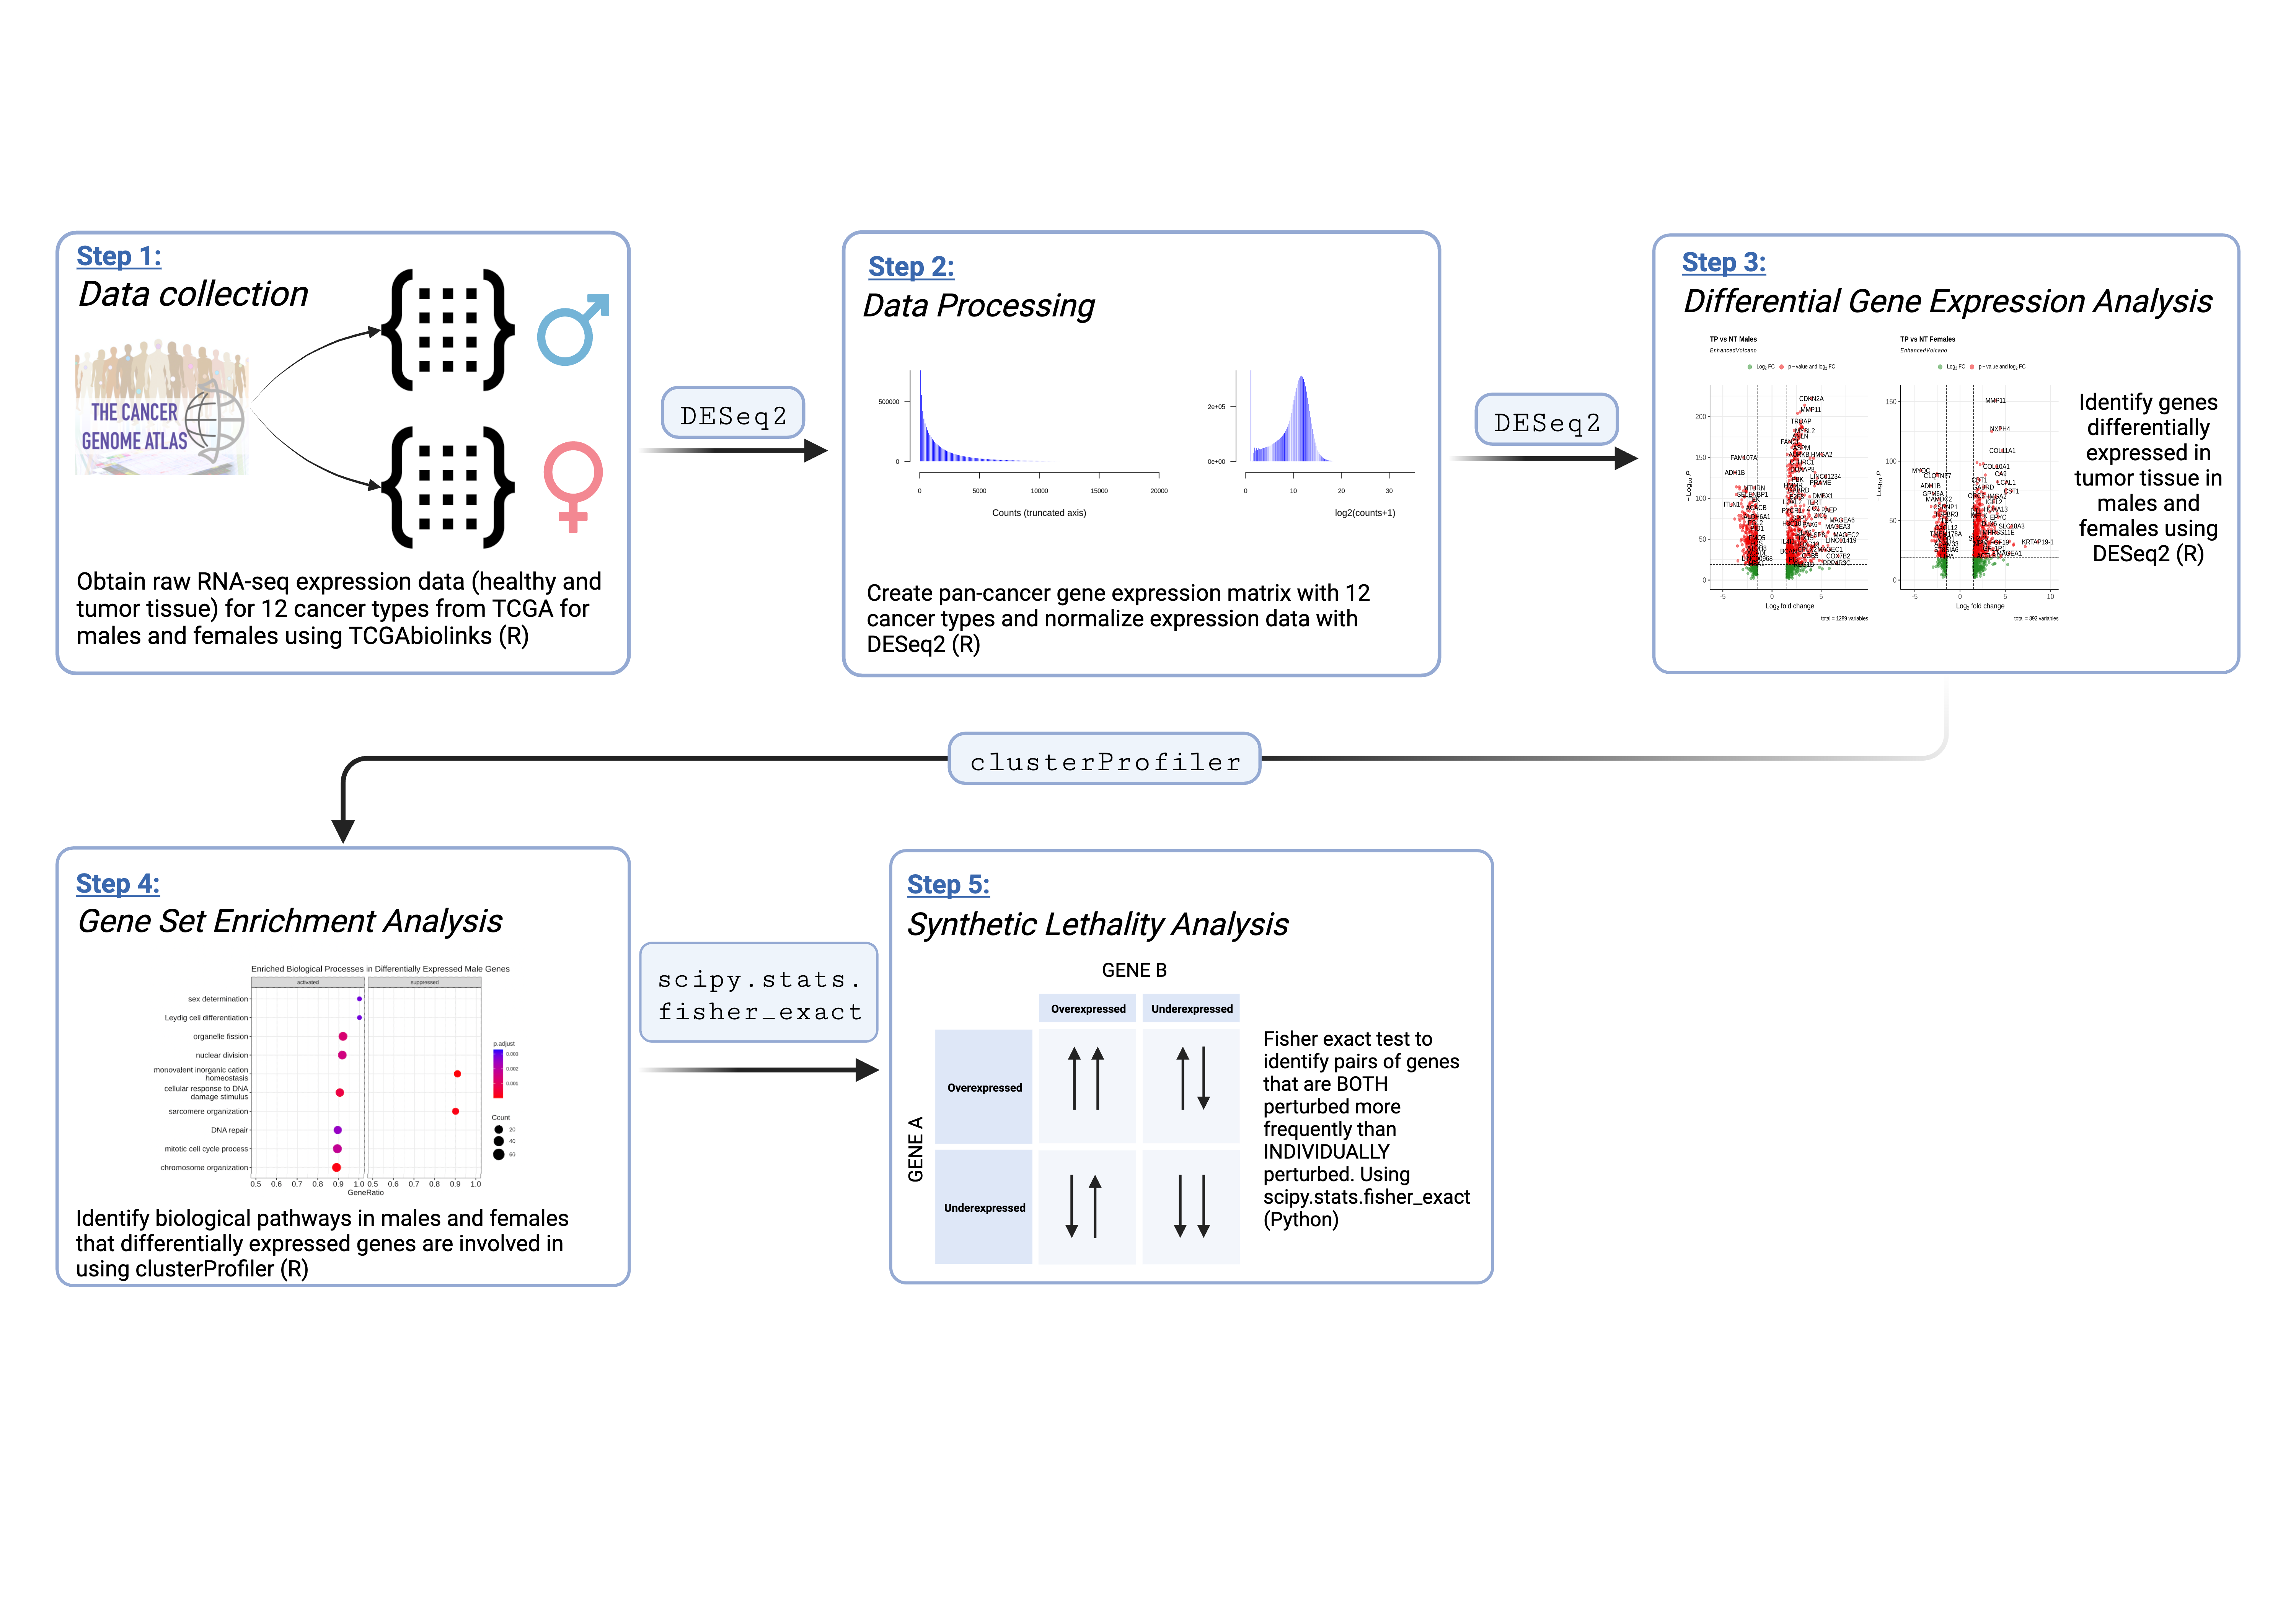
\includegraphics[width=\textwidth, height=13cm]{project_workflow_slpmcrc.png}
\end{center}

\newpage
\section{Introduction/Background Information}

	%What are they
	\subsection{What are Synthetic Lethal Interactions?}

	%Why are they important
	\subsection{Synthetic Lethal Interactions are Harnessed for Precision Oncology}

	%Building SL networks Pan-cancer
	\subsection{Building Pan-Cancer Synthetic Lethality Networks}

	%Bringing sex differences into the paper
	\subsection{Human Sex Differences add An Additional Layer of Complexity}

	%Bringing everything together
	\subsection{Building Pan-Cancer Synthetic Lethality Networks in a Sex Specific Manner} 

\newpage
\section{Materials and Methods} 
%\label{methods}
%Custom scripts and commands utilized in this analysis can be found on \texttt{GitHub} at \url{https://github.com/opticrom/abcmcmc-thesis4c12}.

%\sloppy For a detailed protocol, see Supplementary files on \texttt{GitHub} at
 %\url{https://github.com/JohannaEnright/LCREntropyProject/}.

	\subsection{TCGA Data}
	
	RNA sequencing (RNA-seq) data was obtained from The Cancer Genome Atlas (TCGA). Raw STAR (Spliced Transcripts Alignment to a Reference) aligned counts for tumor tissue and healthy tissue samples were collected. The Cancer Genome Atlas contains genomic information which spans 33 cancer types. For the purpose of this study, only 12 of the 33 cancer types were considered. We first filtered out sex-biased cancers which include breast invasive carcinoma (BRCA), cervical cell carcinoma (CESC), ovarian serous cystadenocarcinoma (OV), prostate adenocarcinoma (PRAD), testicular germ cell tumors (TGCT), uterine corpus endometrial carcinoma (UCEC), and uterine carcinosarcoma (UCS). The reason for this was due to the fact that we are already aware of sex biases in these cancer types. Next, we filtered out blood cancers as well as cancers which lacked normal tissue gene expression samples. This included adrenocortical carcinoma (ACC), lymphoid neoplasm diffuse large b-cell lymphoma (DLBC), glioblastoma multiforme (GBM), acute myeloid leukemia (LAML), and brain lower grade glioma (LGG). The reason for this was due to the fact that we did not have adequate control samples to compare to tumor samples. Finally, we filtered out cancers that did not have any matching pairs of samples (NT and TP from same individual), as well as cancers that had less than 10 matched sample pairs across both males and females. This included mesothelioma (MESO), skin cutaneous melanoma (SKCM), thymoma (THYM), uveal melanoma (UVM), cholangiocarcinoma (CHOL), pancreatic adenocarcinoma (PAAD), pheochromocytoma and paraganglioma (PCPG), rectum adenocarcinoma (READ), and sarcoma (SARC). We selected matched tumor-normal sample pairs to help control for genetic background and other individual-specific factors that could influence gene expression. Once cancer types were selected, two pan-cancer raw count gene expression matrices were created, one for males and one for females.
	
	\begin{table}[ht]
	\centering
	\caption{List of 12 TCGA Cancer Types With Number of Matched Tumor-Normal Samples in Males and Females.}
	% Second version of table, with booktabs.
	\begin{tabulary}{\textwidth}{CCCC}\toprule
		& \multicolumn{3}{c}{TCGA information}
		\\\cmidrule(lr){2-4}
		& Cancer Type  & Matched Female Samples & Matched Male Samples\\\midrule
		& BLCA & 9 & 10 \\
		& COAD & 21 & 20 \\
		& ESCA & 5 & 8 \\
		& HNSC & 14 & 29 \\
		& KICH & 12 & 13 \\
		& KIRC & 20 & 52 \\
		& KIRP & 10 & 22 \\
		& LIHC & 22 & 28 \\
		& LUAD & 34 & 24 \\
		& LUSC & 14 & 37 \\
		& STAD & 10 & 23 \\
		& THCA & 42 & 17 \\
		& \textcolor{red}{TOTAL} & \textcolor{red}{213} & \textcolor{red}{283} \\\bottomrule
	\end{tabulary}
	\end{table}

	\subsection{Pre-filtering and Normalization of Raw RNA-seq Count Data}
	
	Raw count gene expression matrices for males and females were pre-filtered to remove genes unlikely to exhibit differential expression. For each matrix, we calculated the 90th quantile of overall gene expression as a threshold. For each gene in the matrix, we checked to see whether its expression was greater than the threshold in at least 1 sample. We removed genes where no samples showed an expression value greater than the quantile threshold. 
	
	The pre-filtered matrices were then normalized using the \texttt{DESeq2} package in R \citep{love2014moderated}. RNA-seq data must be normalized in order to account for factors that prevent the direct comparison of expression measures. The \texttt{DESeq2} package employs a median of ratios normalization method to account for the inherent biases associated with RNA-seq data. Both sequencing depth (\# of reads generated per sample) and RNA composition (differences in composition of RNA molecules in a sample) are factors accounted for by the \texttt{DESeq2} package. Raw counts are divided by size factors determined for each sample by computing the median ratio of gene counts relative to the geometric gene calculated per gene \citep{love2014moderated}. \figref{fig:1} summarizes the effects of normalization for both male and female RNA-seq data. The distribution of counts across samples becomes much more consistent, thus making the samples comparable.
	
	\begin{figure}[!h]
		\centering	
		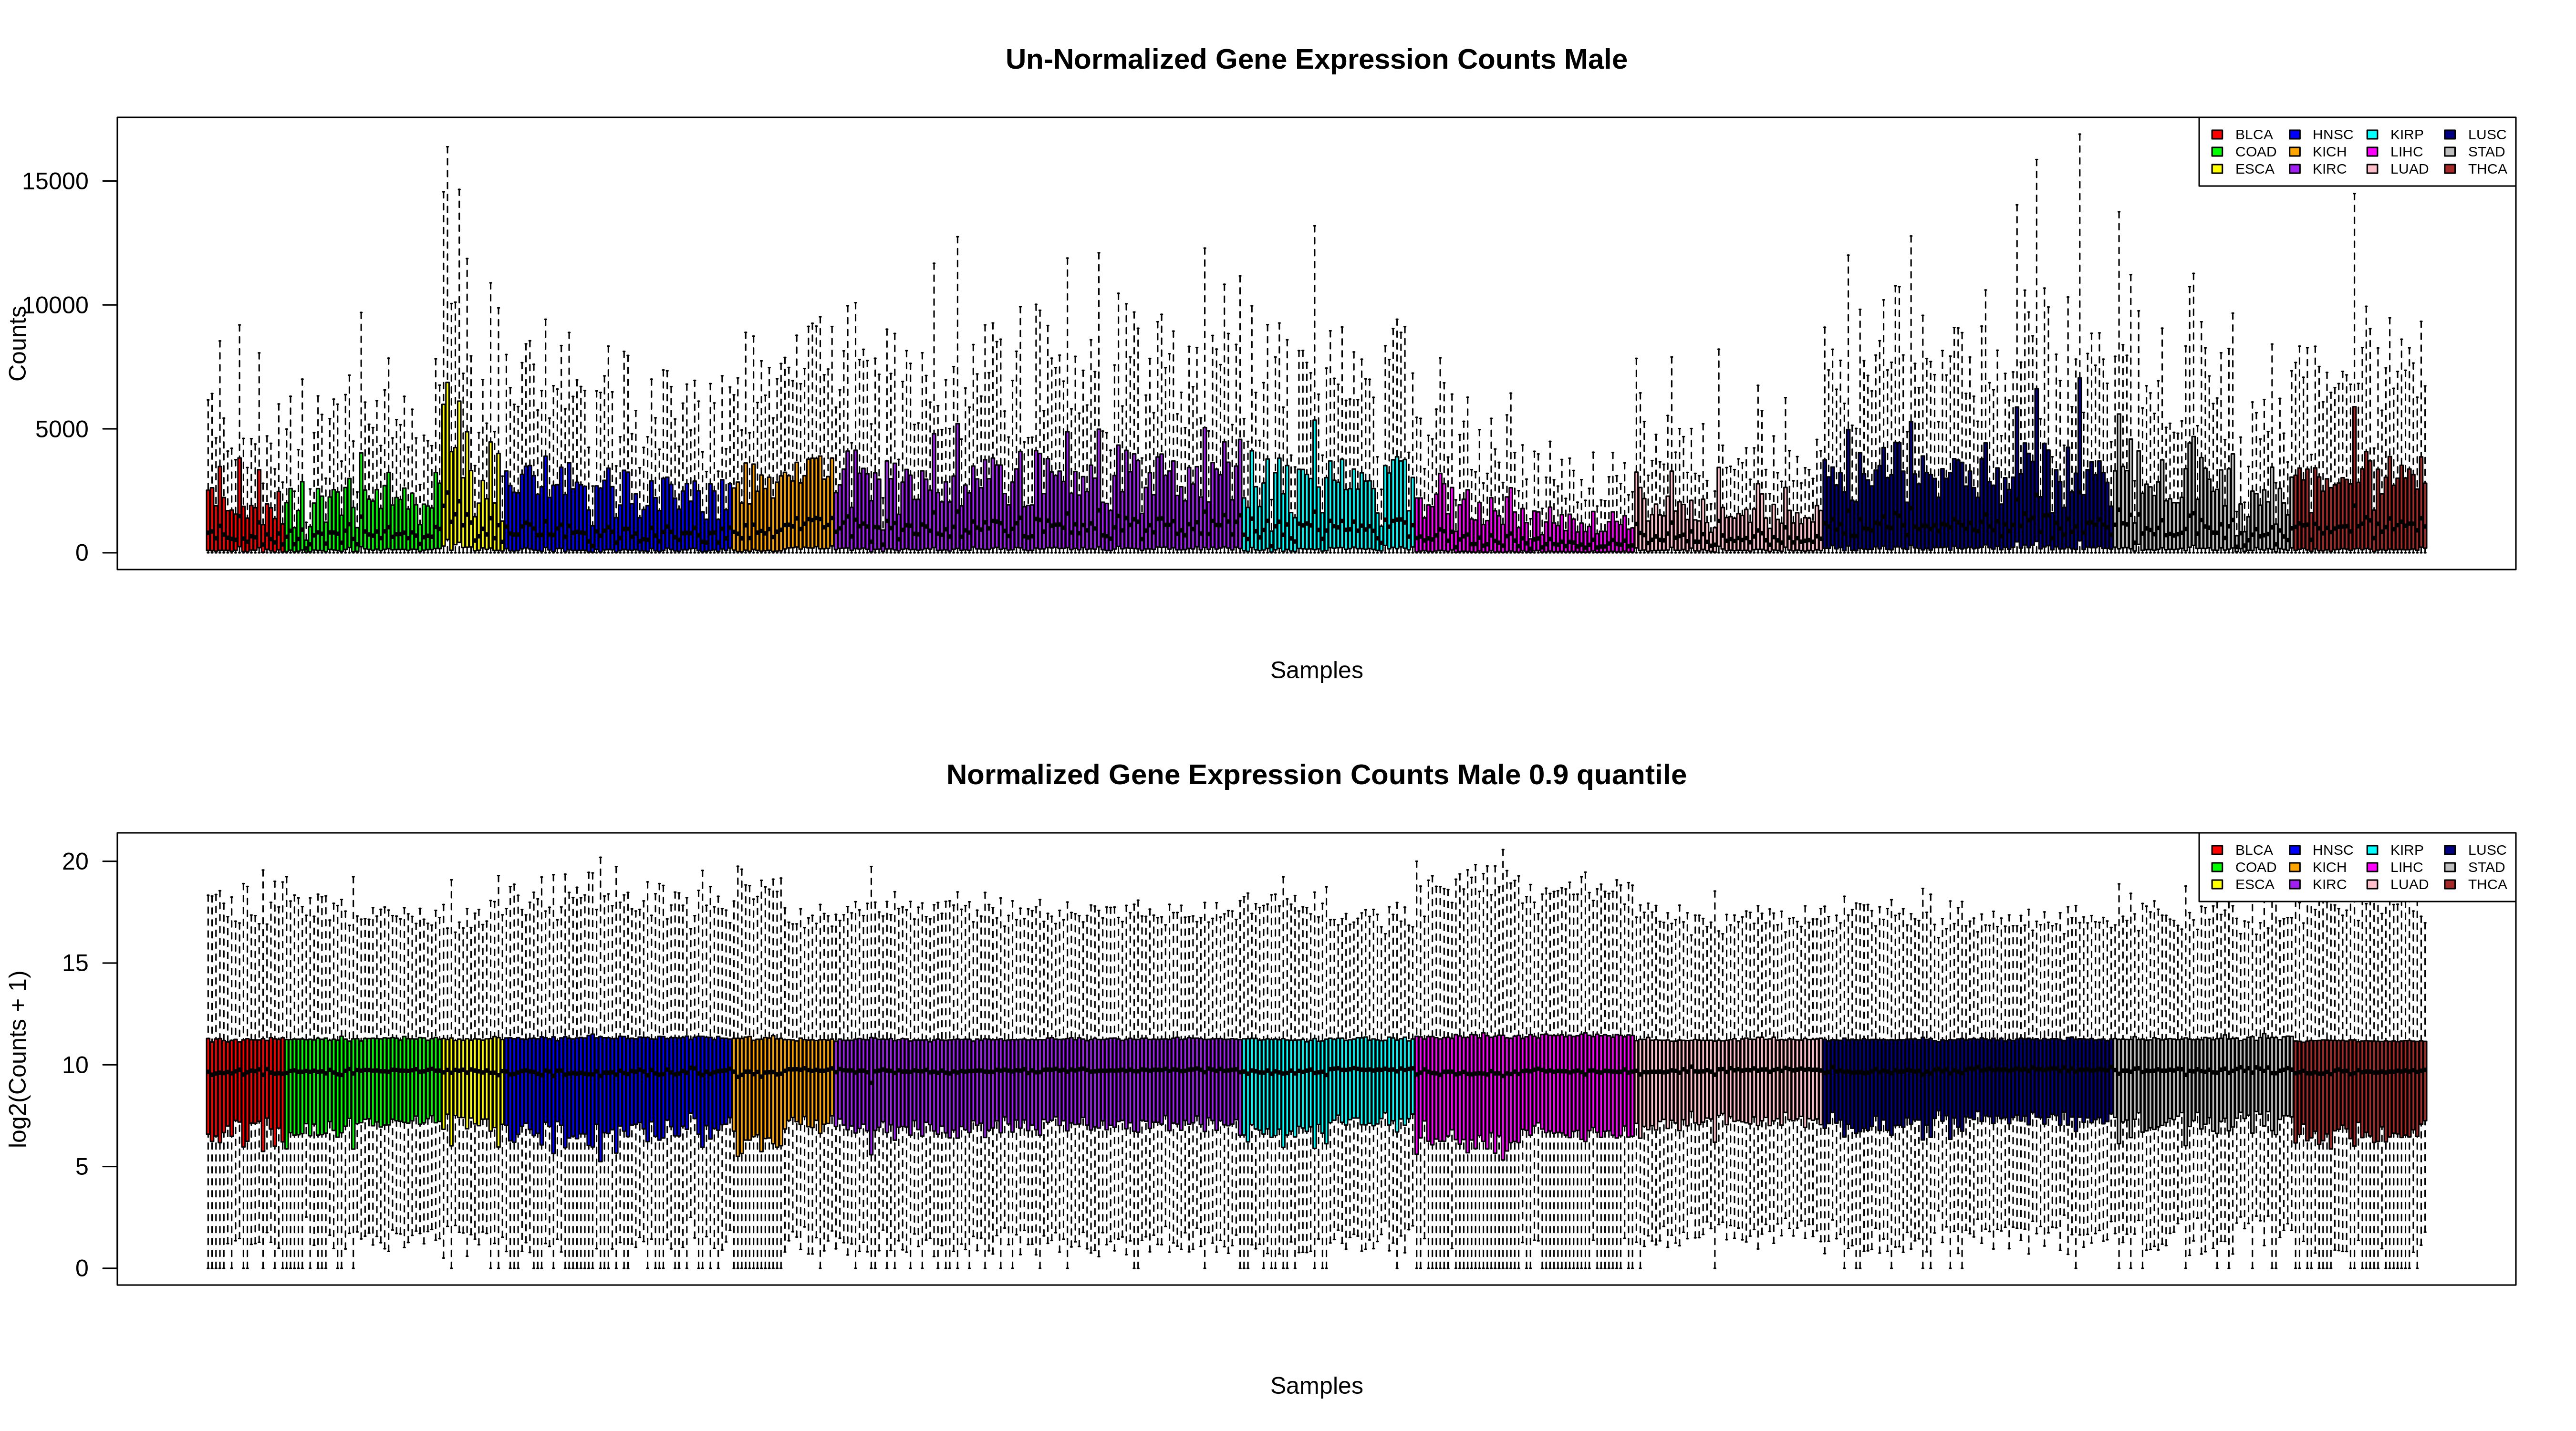
\includegraphics[width=8.5cm, height=6cm]{normalied_male.png}\hfill
		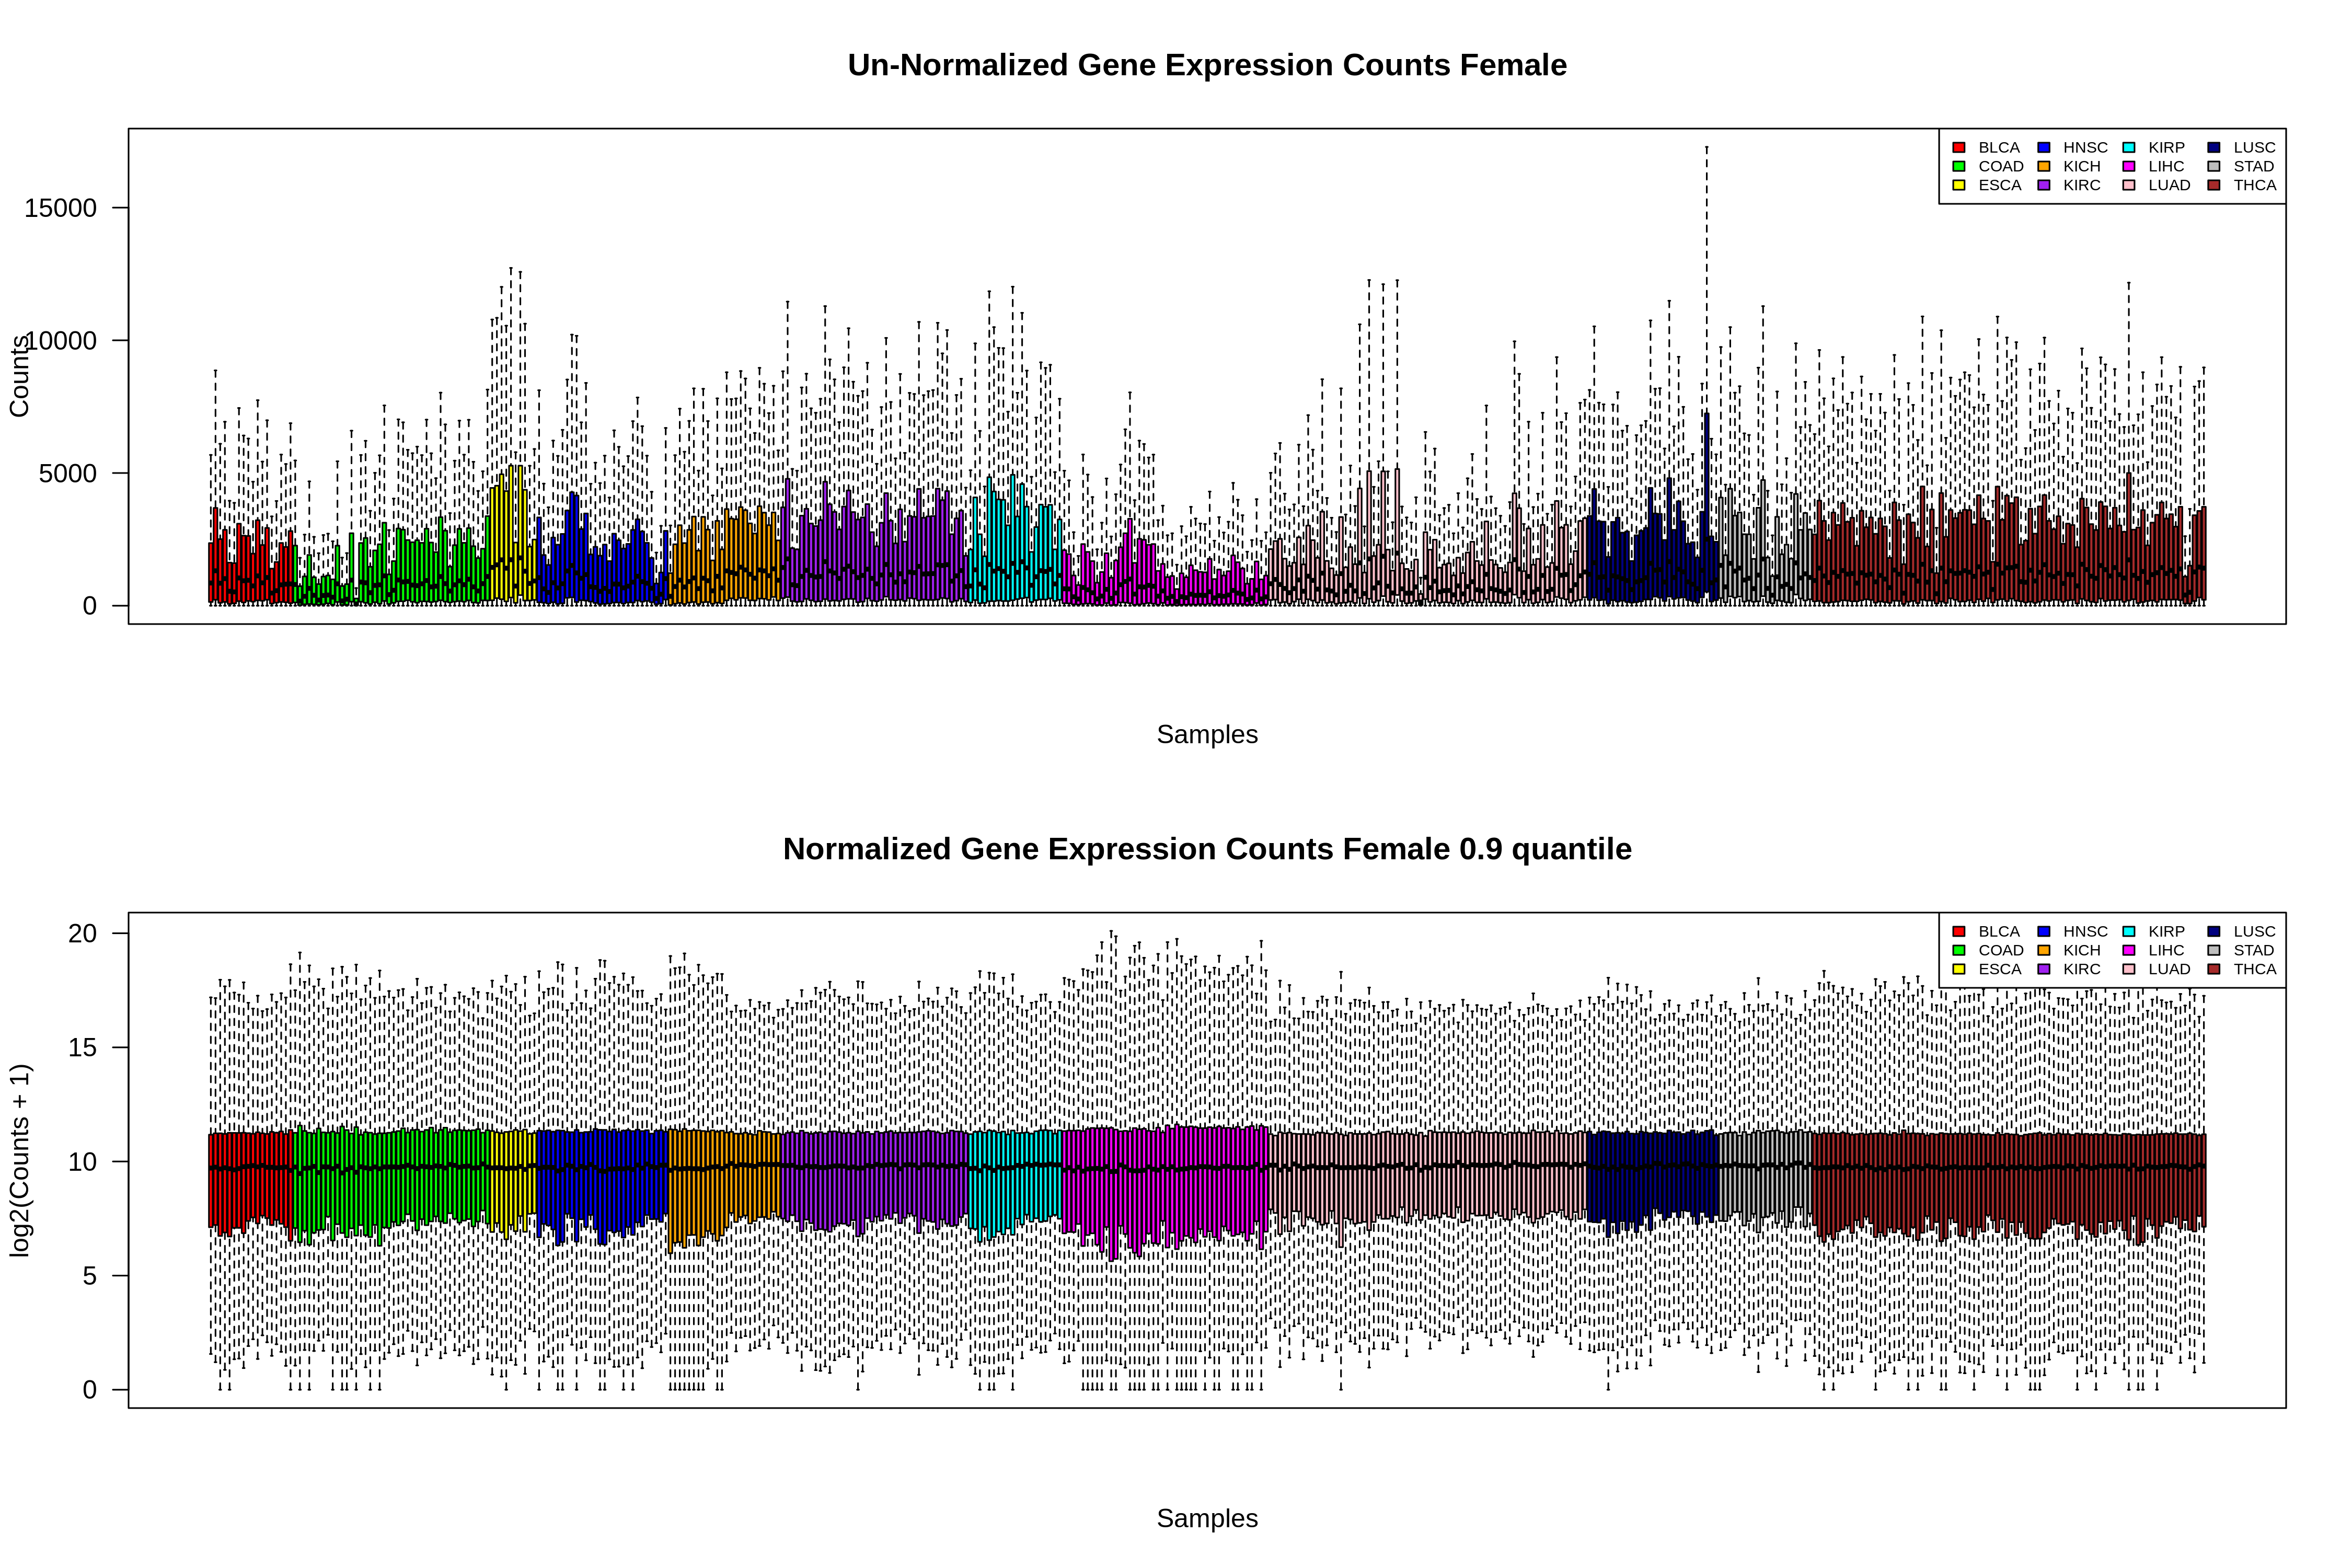
\includegraphics[width=8.5cm, height=6cm]{normalied_female.png}
		\caption{Boxplots highlighting the distribution of raw RNA-seq data (top row) vs normalized RNA-seq data (bottom row) in males (left) and females (right) across normal tissue and tumor tissue samples from 12 TCGA cancer types. Each colour represents a specific cancer type.}
		\label{fig:1}
	\end{figure}

	\subsection{Data Quality Assessment (PCA, NPManova)}
	
	Once expression matrices were normalized, we performed principle component analysis (PCA) on the normalized counts to gain insights into potential factors contributing to the overall variance. Gene expression data is complex due to large number of variables (genes) present. PCA is a technique used to reduce dimensionality by transforming the data to a new set of variables (principle components) that summarize features of the data \citep{yeung2001principal}. In the context of this study, PCA is useful because it can take expression information from many genes, and reduce it down to fewer dimensions, making the data easier to explore. Using PCA, we explored the effects of tissue condition (normal vs tumor), and cancer type on gene expression. 

	\begin{figure}[!h]
		\centering	
		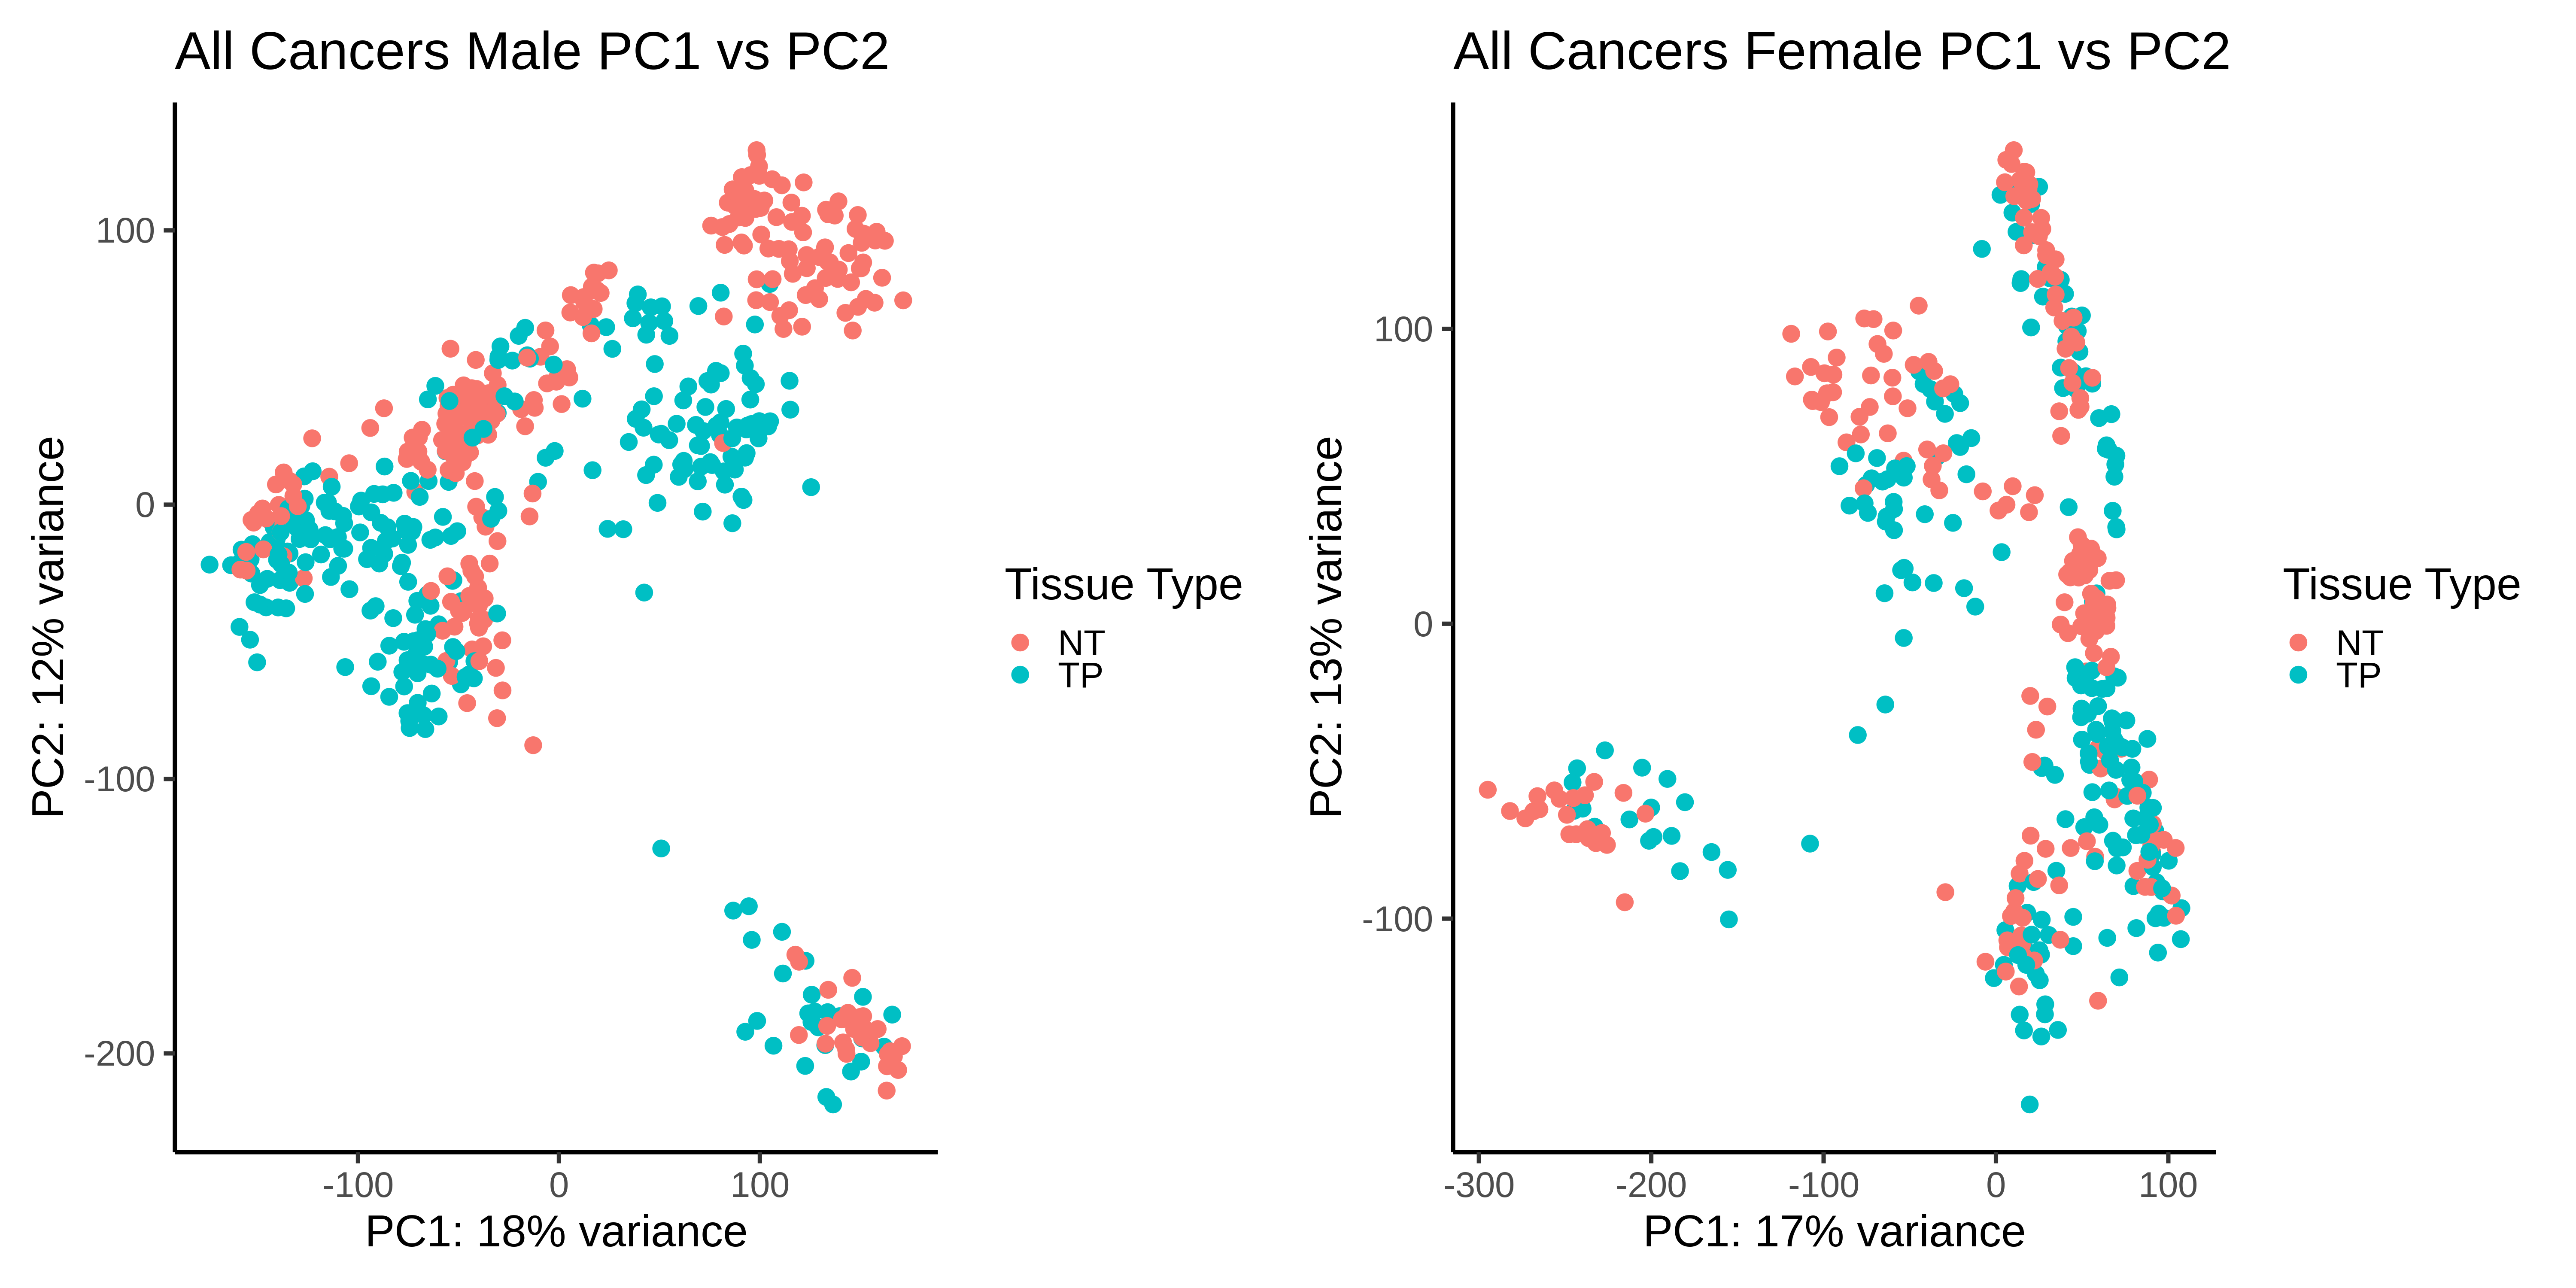
\includegraphics[width=\textwidth,height=9cm]{all_cancerspca_analysis_condition_0.9.png}
		\caption{PCA plot highlighting the effect of tissue condition (normal vs tumor) on gene expression in males (left) and females (right) across 12 cancer types. Normal tissue samples are shown in red, tumor tissue samples are shown in blue.}
		\label{fig:2}
	\end{figure}

	\figref{fig:2} shows the effects of tissue condition (normal vs tumor) on gene expression across the 12 cancer types that were considered in this study. In both males and females, clusters based on tissue condition were present, however there was more variability in clusters of tumor tissue samples compared to clusters of normal tissue samples. \figref{fig:3} shows the effects of both tissue condition and cancer type on gene expression.
	
	\begin{figure}[!h]
		\centering	
		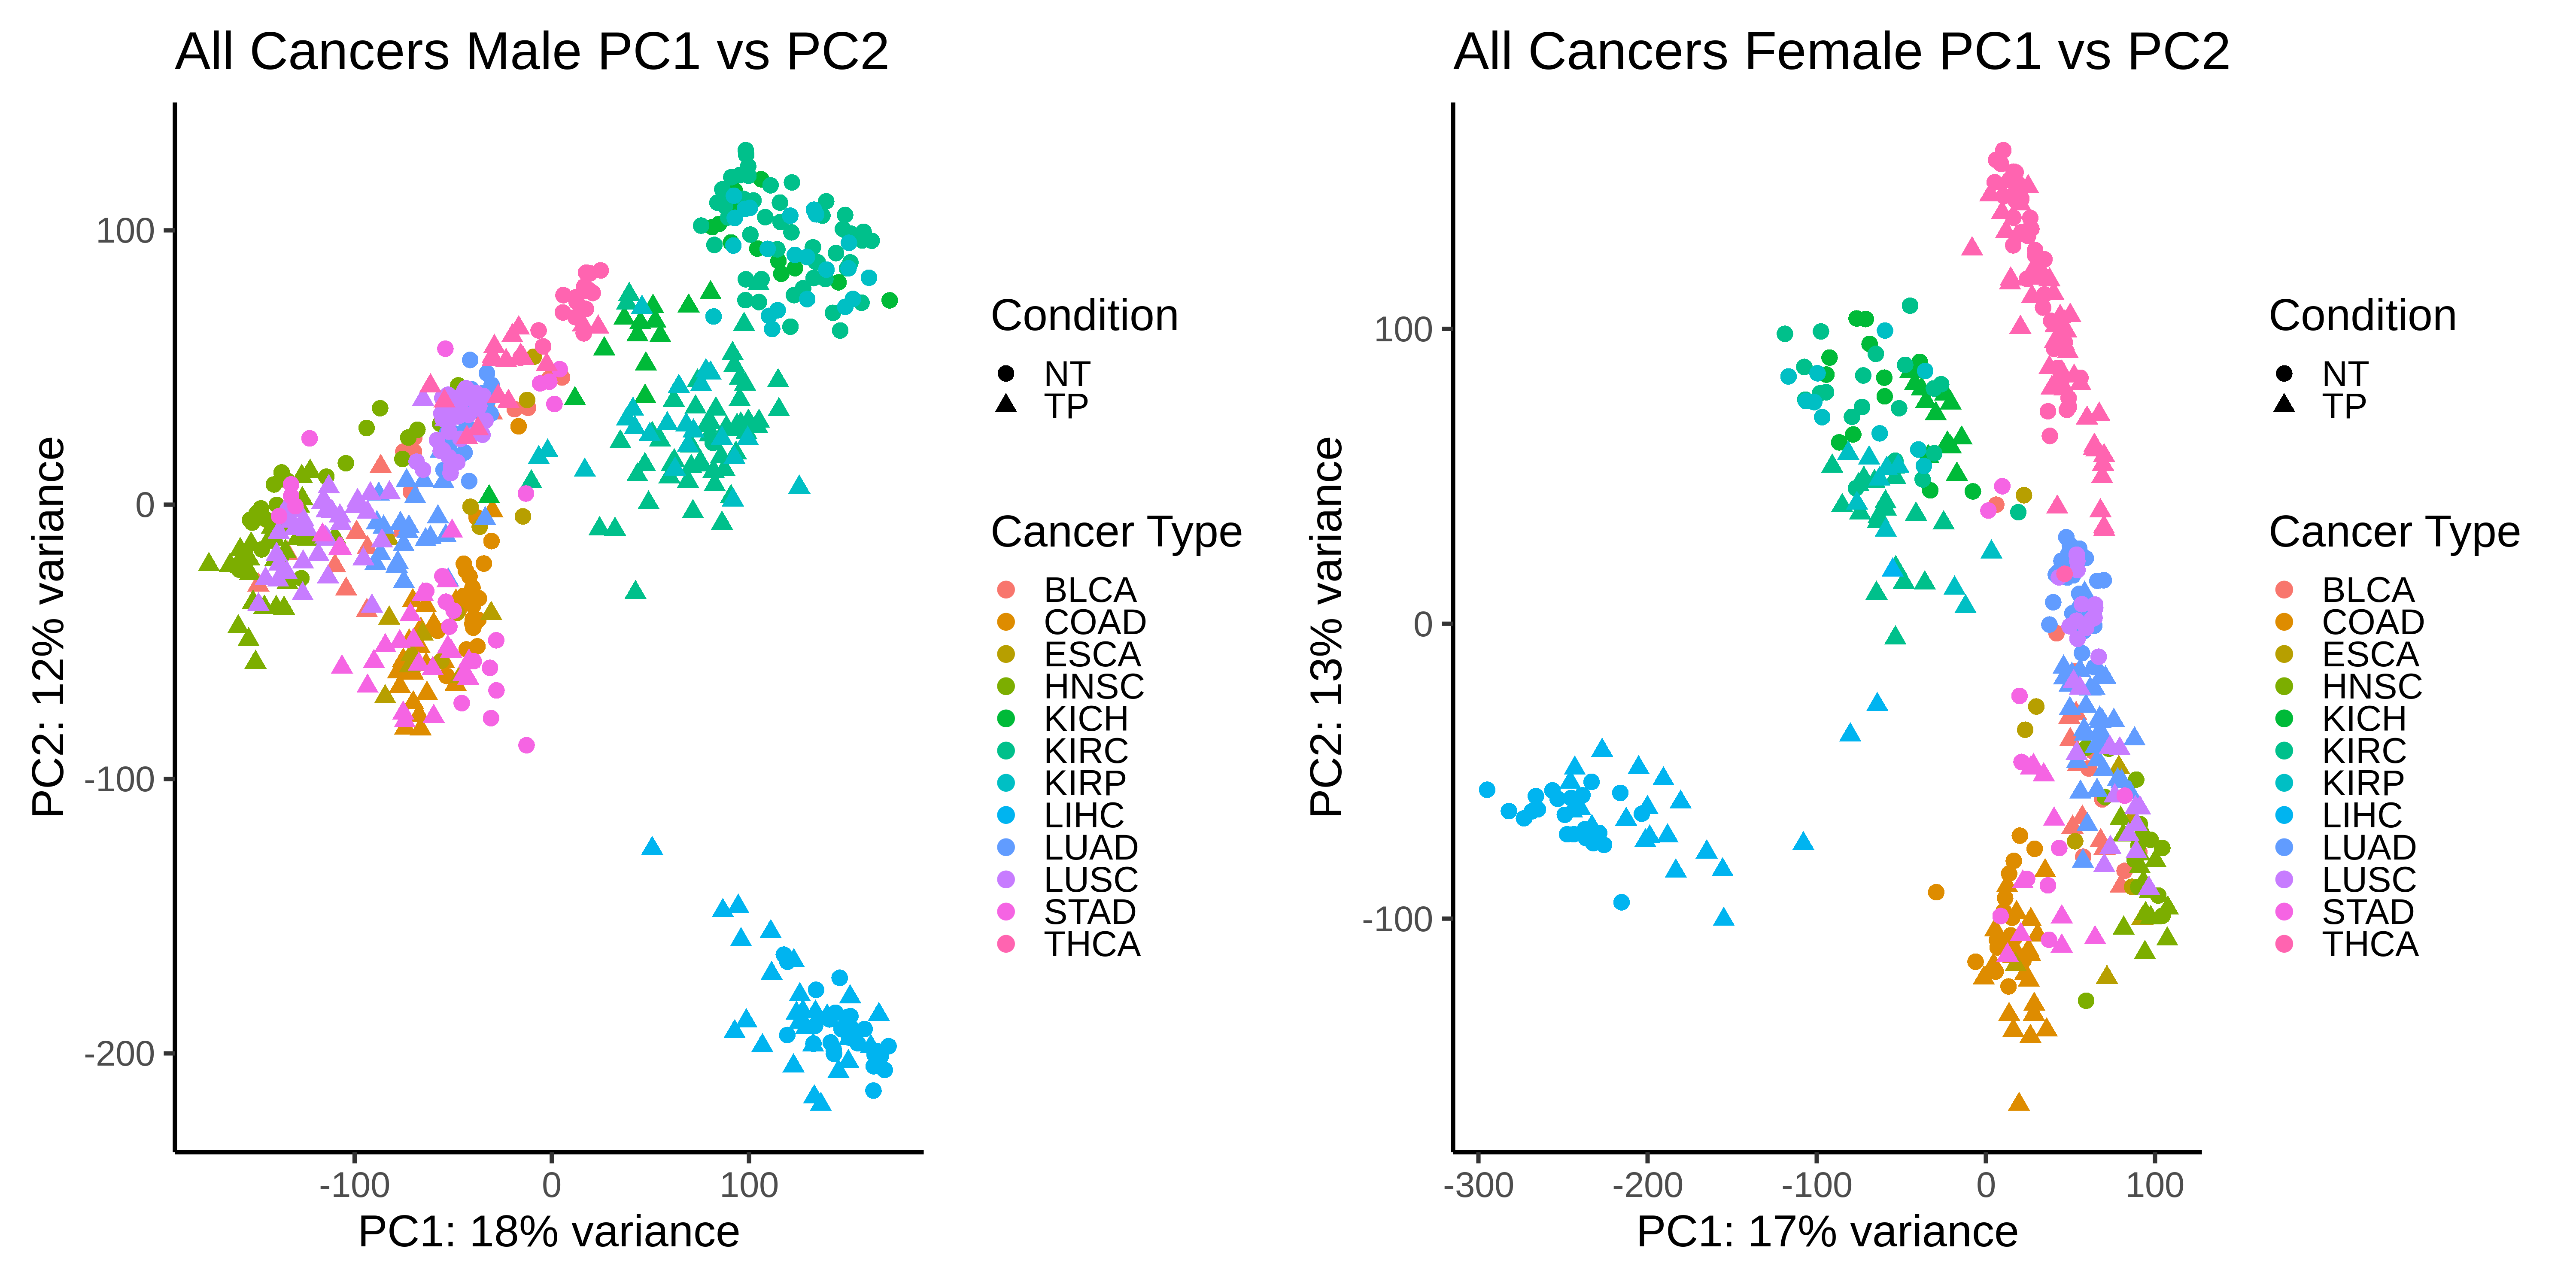
\includegraphics[width=\textwidth,height=9cm]{all_cancerspca_analysis_condition_cancertype_0.9.png}
		\caption{PCA plot highlighting the effect of tissue condition (normal vs tumor) and cancer type on gene expression in males (left) and females (right) across 12 cancer types.}
		\label{fig:3}
	\end{figure}
	
	When we added cancer type as a factor, we obtained much clearer clusters in the PCA plot, suggesting that cancer type is a factor that contributes to the variation in gene expression. We wanted to examine factors that contribute to this variance as these factors may influence which genes are found to be differentially expressed. 
	
	We also verified the statistical significance of the difference between normal and tumor tissue expression across all cancer types and within each cancer type using a non-parametric multivariate analysis of variance (NPMANOVA), also known as a permutational multivariate analysis of variance (PERMANOVA). This is a nonparametric test used to compare multivariate distributions of several groups and the null hypothesis for this test is that the centroids of all groups are equal \citep{anderson2005permutational}. In the case of this study, a low p-value indicates a significant difference in the centroids between normal tissue and tumor tissue. We did not have time to produce PCA plots that showed the centroids, but it would be beneficial to produce these plots in the future. We also did not perform an analysis that could identify the variance among the clusters so we could not statistically test if there was more heterogeneity among tumor tissue samples compared to normal tissue samples. \newline
	
	\begin{table}[!h]
		\centering
		\vspace{-0.2cm}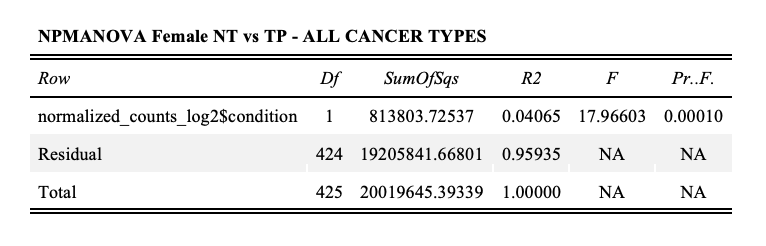
\includegraphics[width=18cm, height=5cm]{allfemale_npmanova.png}
		\caption{Results from one-way NPMANOVA comparing centroids of normal tissue and tumor tissue gene expression in females across all 12 cancer types considered in the study}
		\label{table:2}
	\end{table}

	\begin{table}[!h]
		\centering
		\vspace{-0.2cm}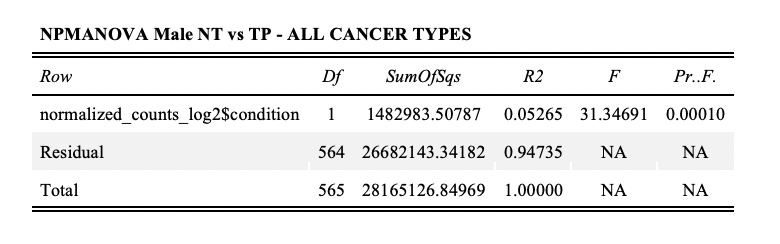
\includegraphics[width=18cm, height=5cm]{allmale_npmanova.png}
		\caption{Results from one-way NPMANOVA comparing centroids of normal tissue and tumor tissue gene expression in males across all 12 cancer types considered in the study}
		\label{table:3}
	\end{table}

Table 2 and Table 3 show the results of the one-way NPMANOVA (for females and males respectively) comparing the centroids of tumor tissue and normal tissue expression across all 12 cancer types together. In both males and females, the small p-value indicates a significant difference in normal vs tumor tissue when considering all 12 cancer types collectively.
	
	\begin{table}[!h]
		\centering
		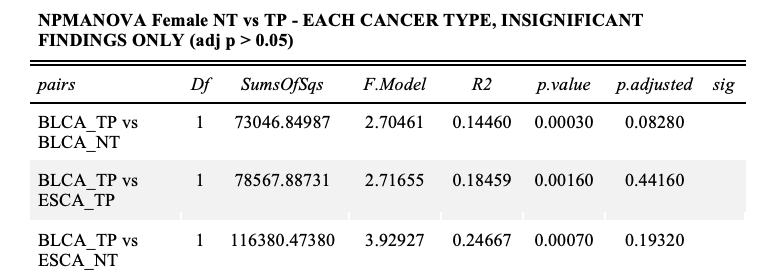
\includegraphics[width=18cm, height=6cm]{eachfemale_npmanova.png}
		\caption{Results from pairwise NPMANOVA comparing centroids of normal tissue and tumor tissue gene expression in females for each individual cancer type considered in the study (full table not shown here)}
		\label{table:4}
	\end{table}

	\begin{table}[!h]
		\centering
		\vspace{-0.4cm}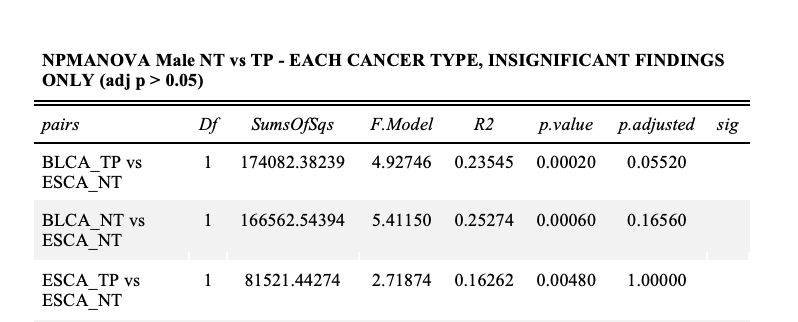
\includegraphics[width=18cm, height=7cm]{eachmale_npmanova.png}
		\caption{Results from pairwise NPMANOVA comparing centroids of normal tissue and tumor tissue gene expression in males for each individual cancer type considered in the study (full table not shown here)}
		\label{table:5}
	\end{table}

	Table 4 and Table 5 show the results of the pairwise NPMANOVA (for females and males respectively) comparing the centroids of tumor tissue and normal tissue expression within each of the 12 cancer types individually. Shown in these tables are insignificant results (pairwise comparisons with adjusted p-value > 0.05) as it is easier to show which comparisons were not considered to be statistically significant. Only 3 rows of each table are shown, not the full tables.

	\subsection{Differential Gene Expression Analysis with DESeq2}
	
	Based on the above analysis, we decided to control for cancer type as it was found to be an important source of variation that could potentially confound the comparison between normal and healthy tissue conditions. We used \texttt{DESeq2} to identify differentially expressed genes \citep{love2014moderated}. \texttt{DESeq2} utilizes the negative binomial distribution (AKA gamma-poisson distribution) to model the expression count data. The reason for using the negative binomial distribution as opposed to using the Poisson distribution (another distribution used to model count data) is due to the negative binomial distributions ability to account for variance (second paramter called dispersion). Typically with RNA-seq data, what we see is that the mean does not equal the variance. \figref{fig:4} shows this relationship and what we see is that the variance increases with mean expression (mean does not equal variance, hence Poisson is a poor choice). 
	
	\begin{figure}[!h]
		\centering
		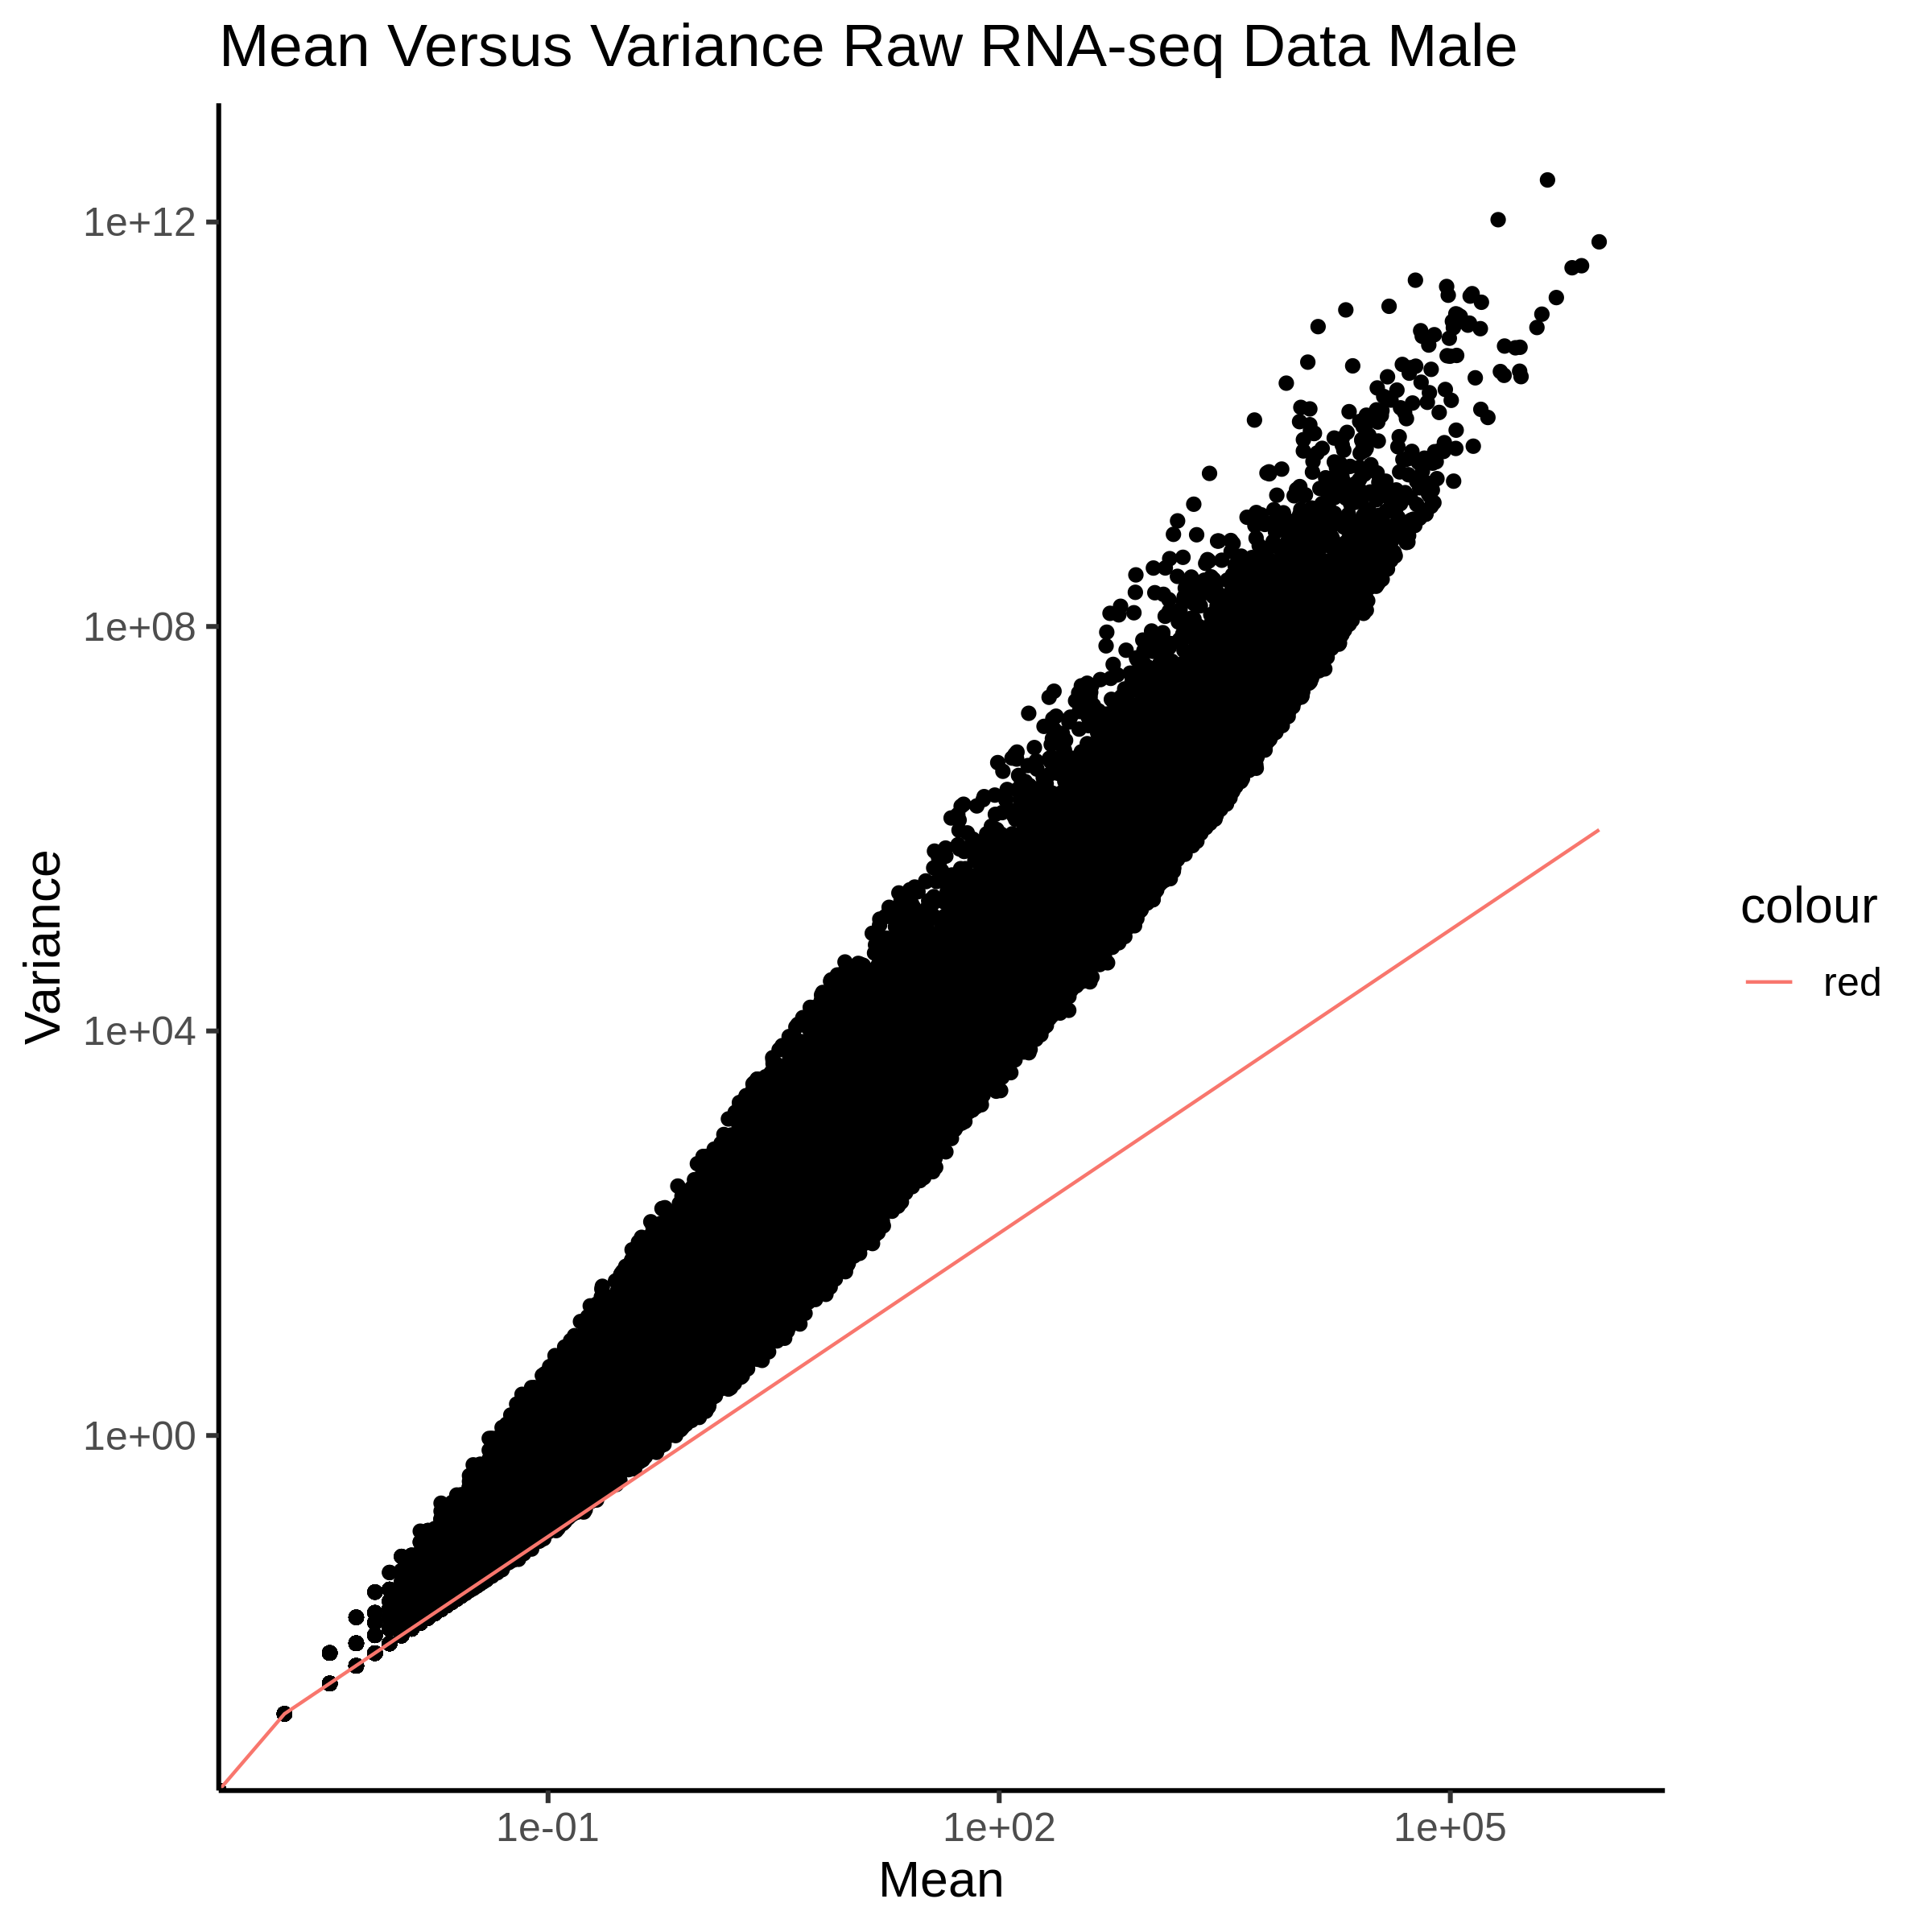
\includegraphics[width=10cm, height=10cm]{all_cancersmean_vs_variance_male.png}
		\caption{Scatter plot showing the mean of gene counts (x-axis) vs variance of gene counts (y-axis) in males for all 12 cancer types considered in the study. The red line shows mean vs mean.}
		\label{fig:4}
	\end{figure}
	
	\texttt{DESeq2} calculates dispersion estimates which accounts for the inherent variability in RNA-seq count data. Once dispersion estimates are calculated for each gene, a negative binomial generalized linear model (GLM) is fit for each gene which incorporates parameters for both mean and dispersion. Once GLM's are fit for each gene, a statistical test called the Wald test is employed to find differentially expressed genes between conditions of interest. Since \texttt{DESeq2} uses a linear model, it gives us the ability to create more complex designs \citep{love2014moderated}. In our analysis, we incorporated cancer type as a factor in the GLM. The following formula below was used by DESeq2 to test the effect of condition (normal vs tumor tissue) while controlling for the effect of cancer type.
	
	\begin{equation}
		design = cancer\_type + condition
	\end{equation}

	Genes found to be significantly differentially expressed were visualized using a volcano plot shown in \figref{fig:5}. Each gene is represented by an individual dot and the colour of the dot represents the gene passing a specific significance threshold. Red dots indicate that the gene had a p-value < 10e-20, and a log2FoldChange > 1.5 or < -1.5 whereas green dots indicate that the gene ONLY had a log2FoldChange > 1.5 or < 1.5. The log2FoldChange is a metric that quantifies the magnitude of change in gene expression between normal and tumor tissue conditions. Dots on the left side of each plot, with a log2FoldChange < -1.5, indicate donwregulation/decreased expression of the gene in tumor tissue compared to normal tissue. Dots on the right side of each plot, with a log2FoldChange > 1.5 indicate upregulation/increased expression of the gene in tumour tissue compared to normal tissue. We set the p-value threshold high when making these volcano plots to minimize the number of genes shown on the plot for aesthetic purposes.
	
	\begin{figure}[!h]
		\centering
		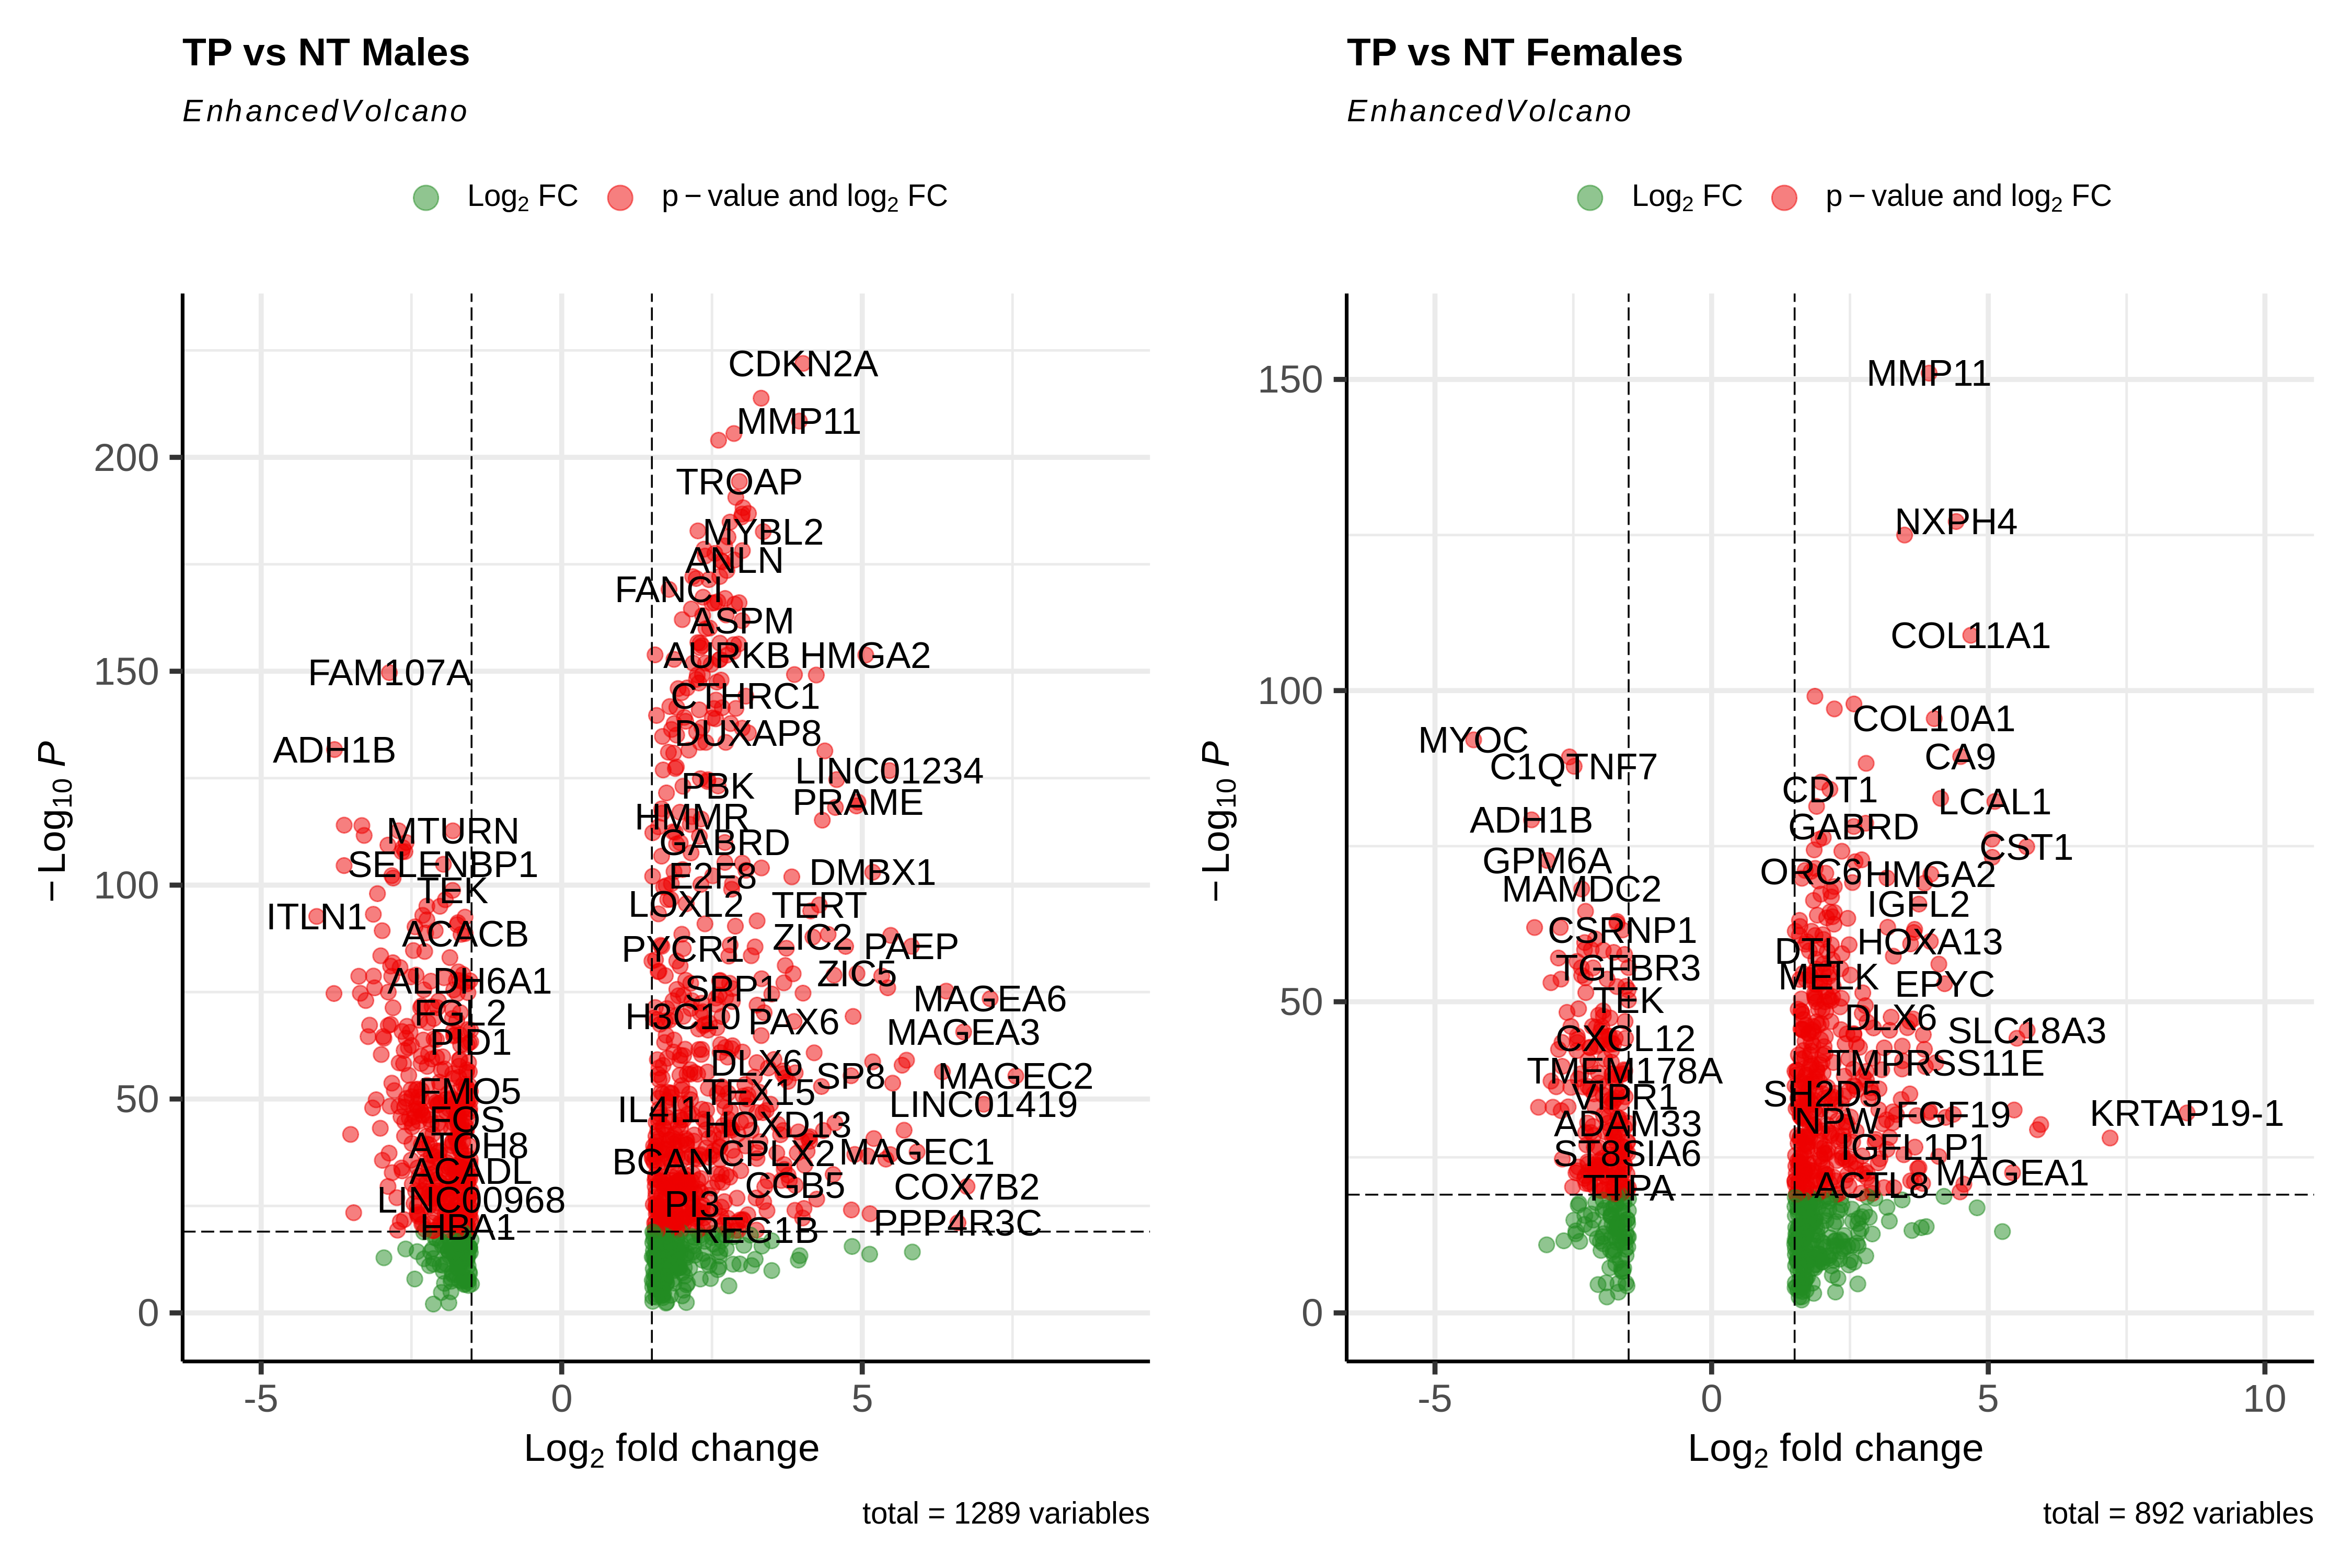
\includegraphics[width=\textwidth, height=12cm]{all_cancersvolcano_analysis_0.9.png}
		\caption{Volcano plot highlighting the genes found to be differentially expressed in tumor tissue compared to normal tissue in males (left) and females (right). A red dot indicates the gene had a p-value < 10e-20 and log2FoldChange > 1.5 or < -1.5. A green dot indicates the gene only had a log2FoldChange > 1.5 or < -1.5}
		\label{fig:5}
	\end{figure}

	The total number of differentially expressed genes are shown below in \figref{fig:6}. We found 1289 male genes to be significantly differentially expressed and 892 female genes to be significantly differentially expressed. (adj p-value < 0.05 AND |log2FoldChange| > 1.5). We compared the differentially expressed genes found in males and females and discovered 651 shared genes, 638 genes found only differentially expressed in males, and 241 genes found only differentially expressed in females. We also determined the number of genes found upregulated and downregulated in tumor tissue. In males, of the 1289 total genes found, 497 were found downregulated in tumor tissue while 792 were found upregulated in tumor tissue. In females, of the 892 total genes found, 287 were found downregulated in tumor tissue and 605 were found upregulated in tumor tissue.
	
	\begin{figure}[!h]
		\centering
		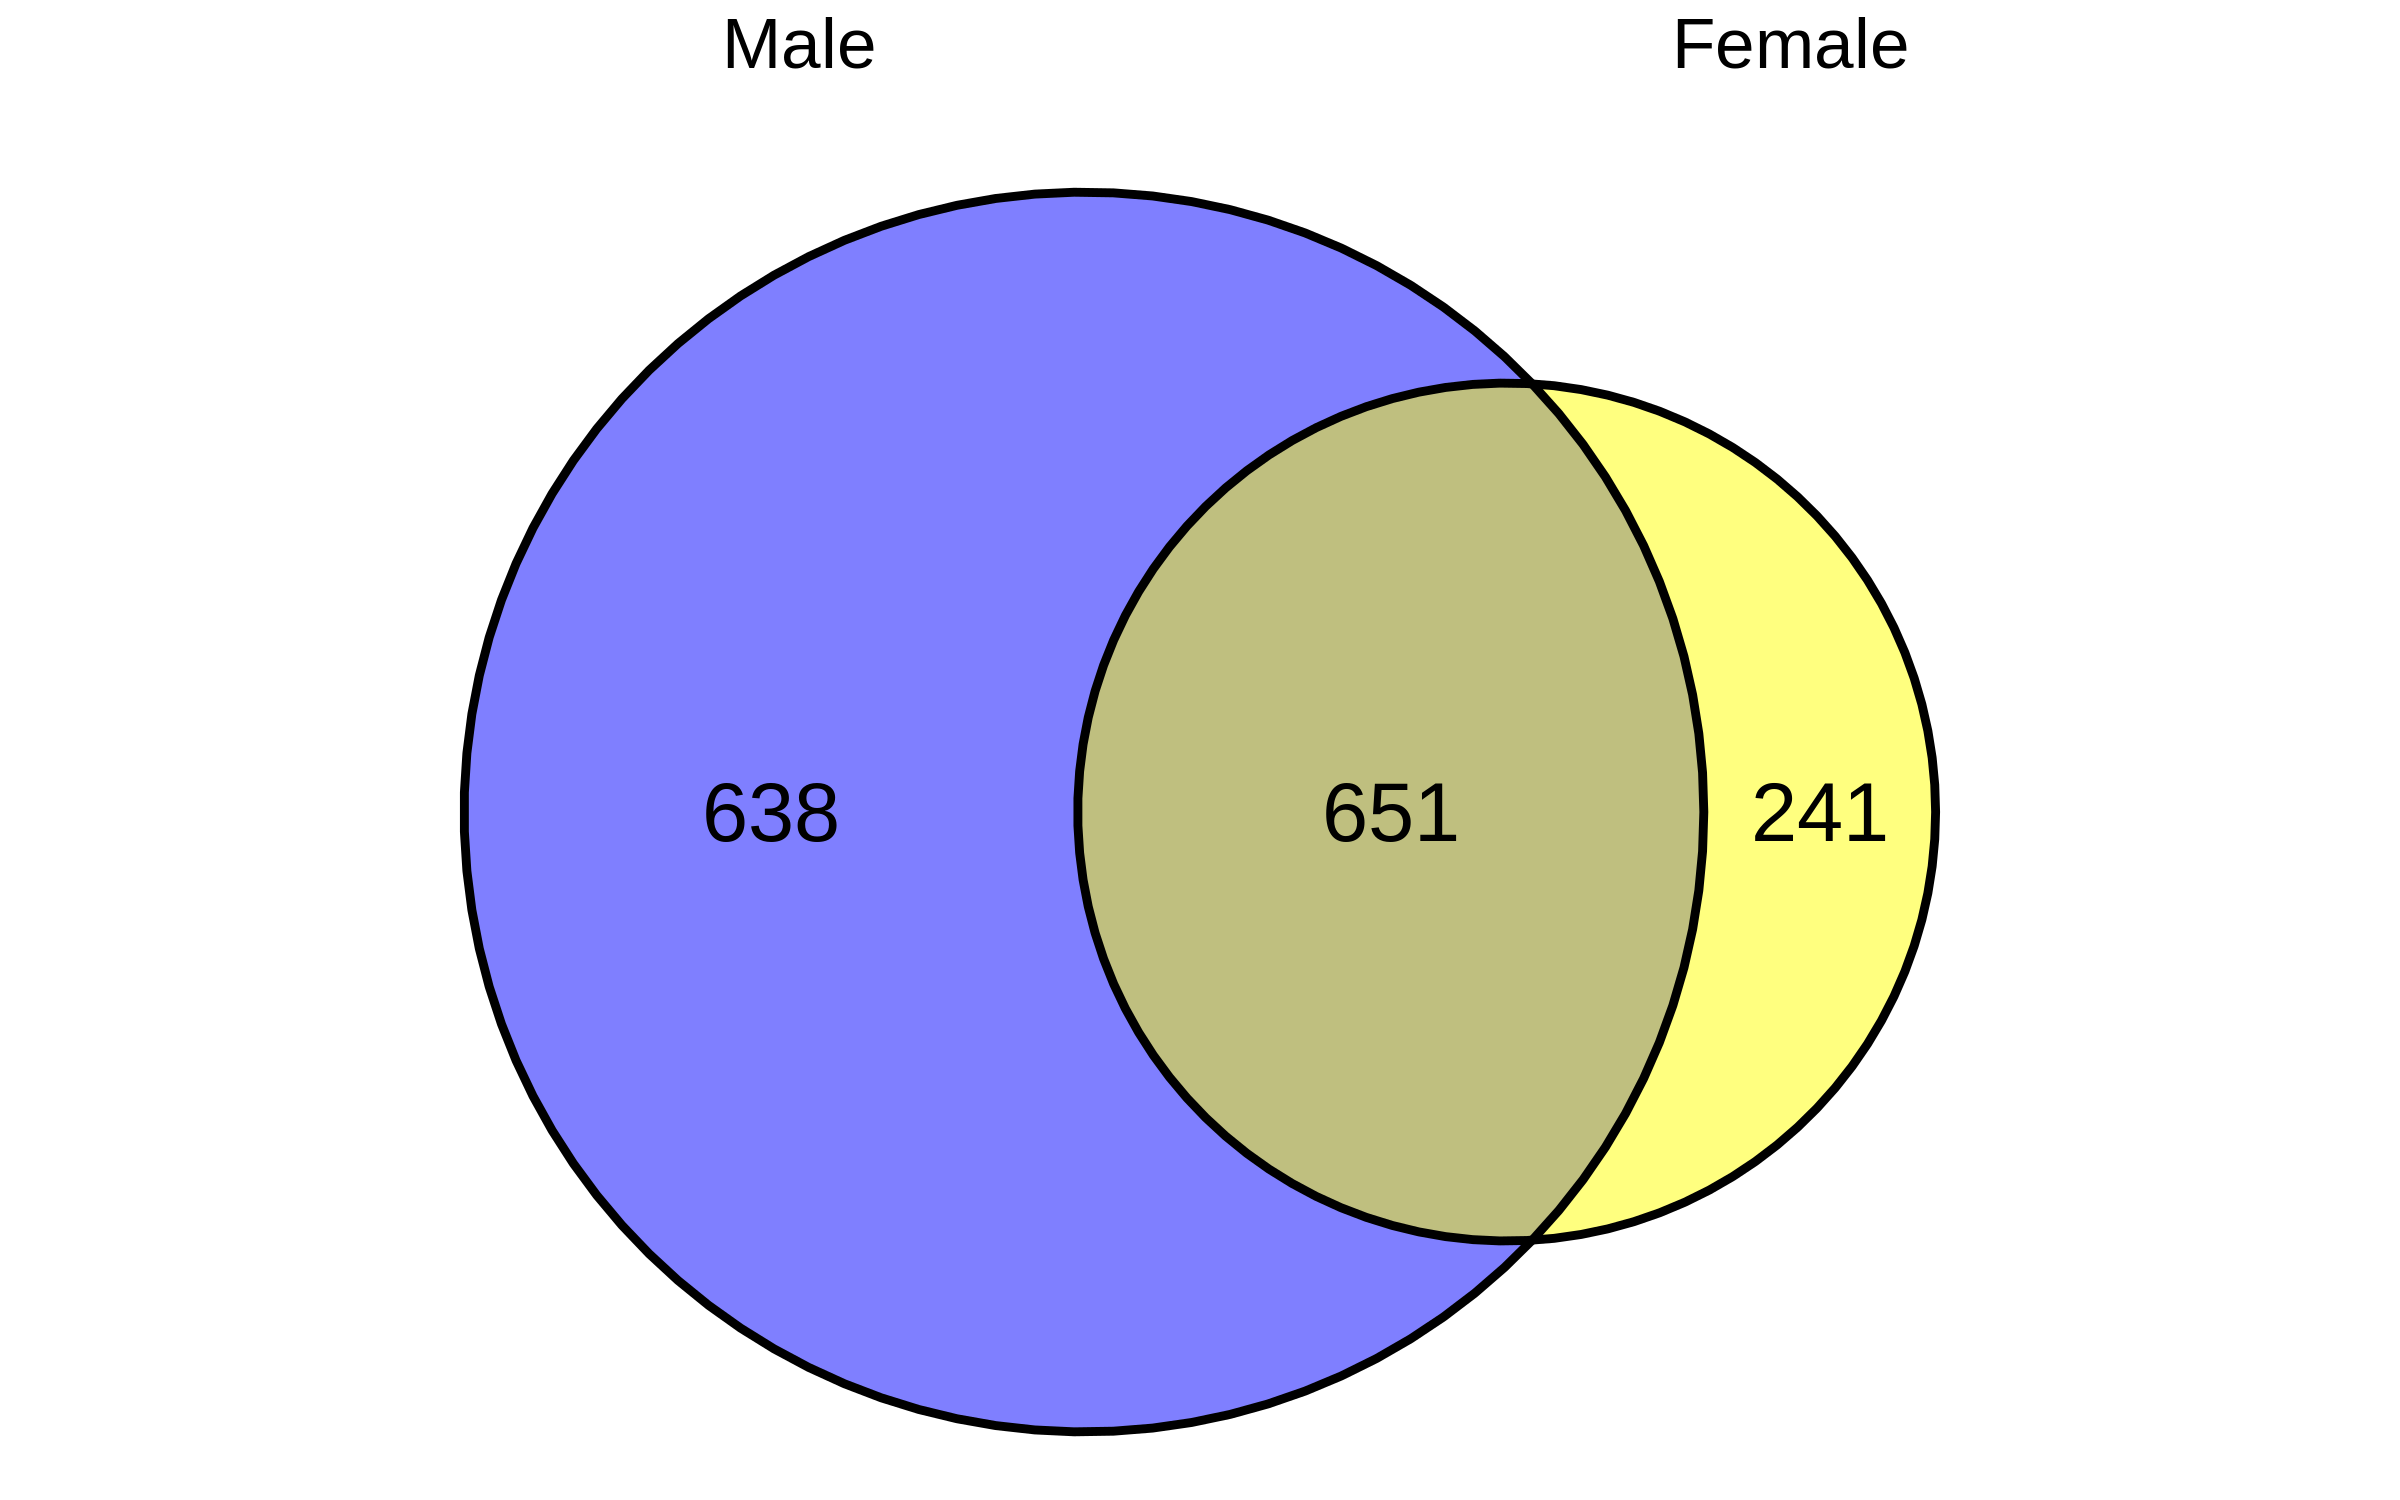
\includegraphics[width=8cm, height=5cm]{all_cancersvenndiagram_malede_vs_femalede_0.9.png}
		\caption{Venn diagram showing the similarities and differences between differentially expressed genes found in males and females}
		\label{fig:6}
	\end{figure}
	
	\subsection{Gene Set Enrichment Analysis with ClusterProfiler}
	
	We used the \texttt{clusterProfiler} R package to perform gene set enrichment analysis (GSEA) in order to gain insight into the functional groups of genes enriched in certain biological pathways. The package depends on annotation data from GO.db (Gene Ontology) and KEGG.db (Kyoto Encyclopedia of Genes and Genomes) in order to calculate enrichment test for GO and KEGG pathways \citep{yu2012clusterprofiler}. Essentially the analysis determines whether members of a gene set (unordered collections of genes that are functionally related) are randomly distributed in a list of differentially expressed genes, or primarily found at the top (overexpressed) or bottom (underexpressed) when sorted based on log2FoldChange \citep{yu2012clusterprofiler}.
	
	\begin{figure}[!h]
		\centering
		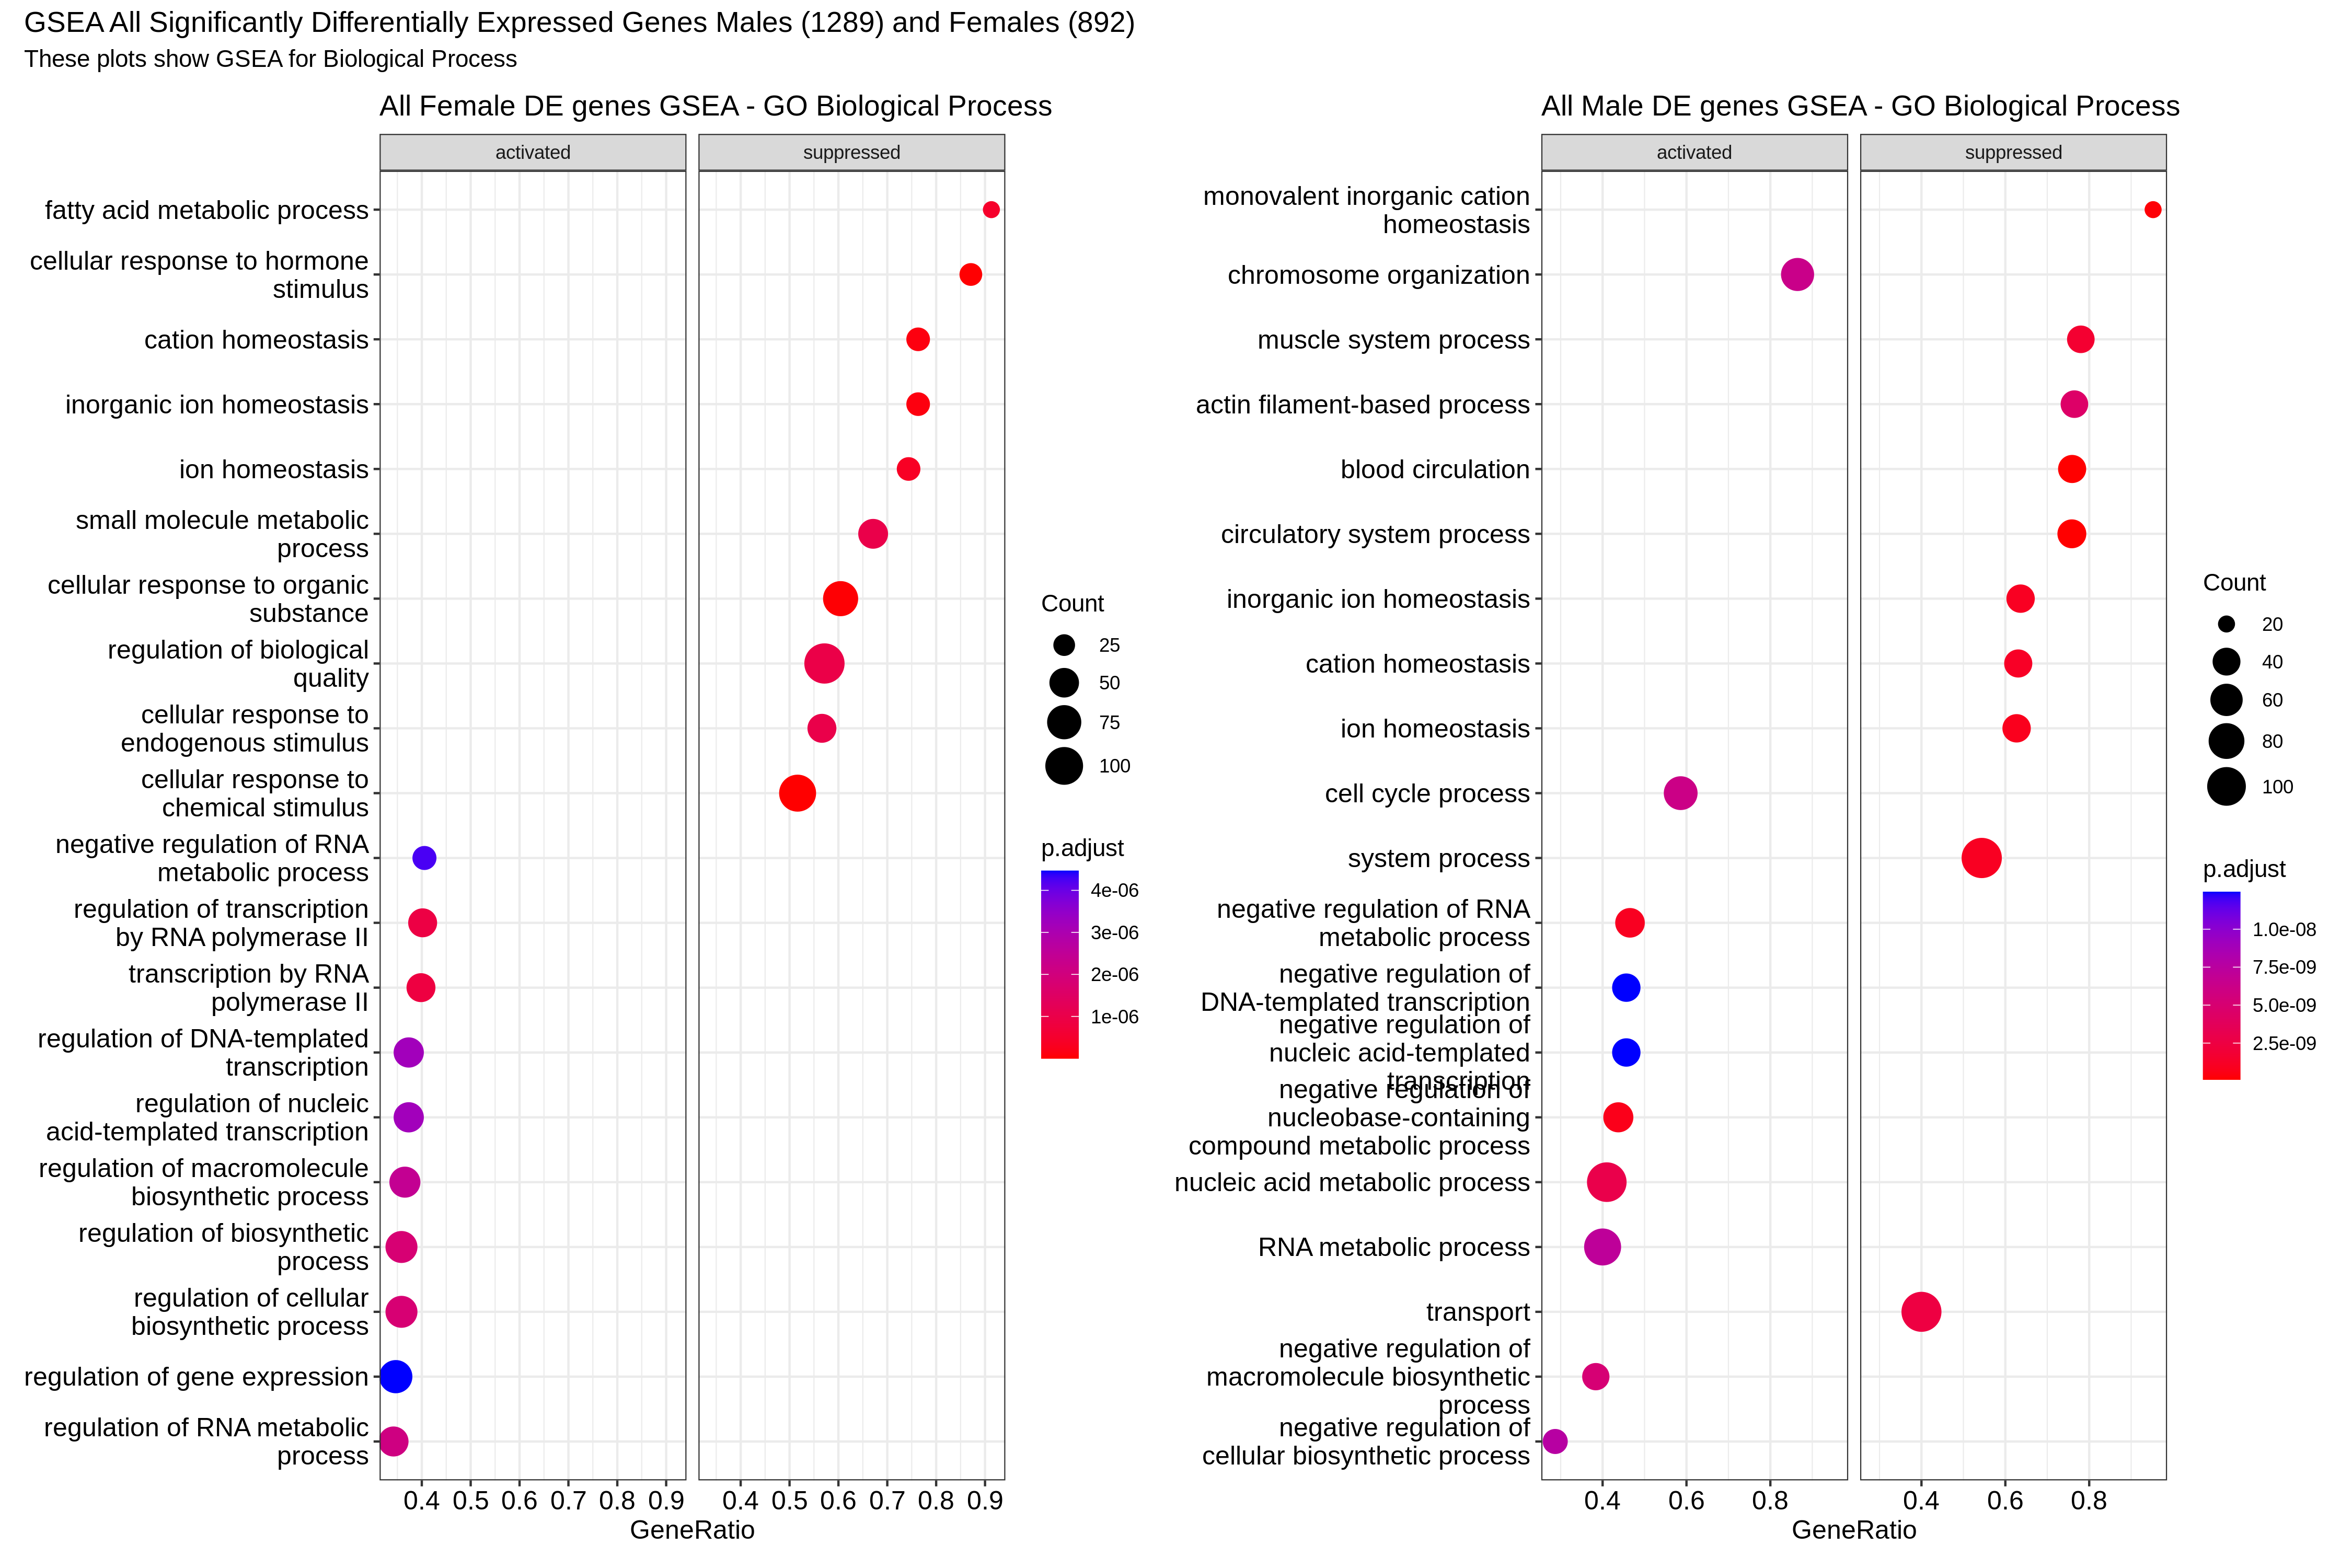
\includegraphics[width=17cm, height=10cm]{all_cancersgsea_alldegenes_male_female_bp0.9.png}
		\caption{Dotplot showing the results of GSEA performed on ALL differentially expressed genes (892 female, 1289 male) found in females (left) and males (right). This example shows 10 activated and 10 suppressed enriched gene sets.}
		\label{fig:7}
	\end{figure}
		
	\begin{figure}[!h]
		\centering
		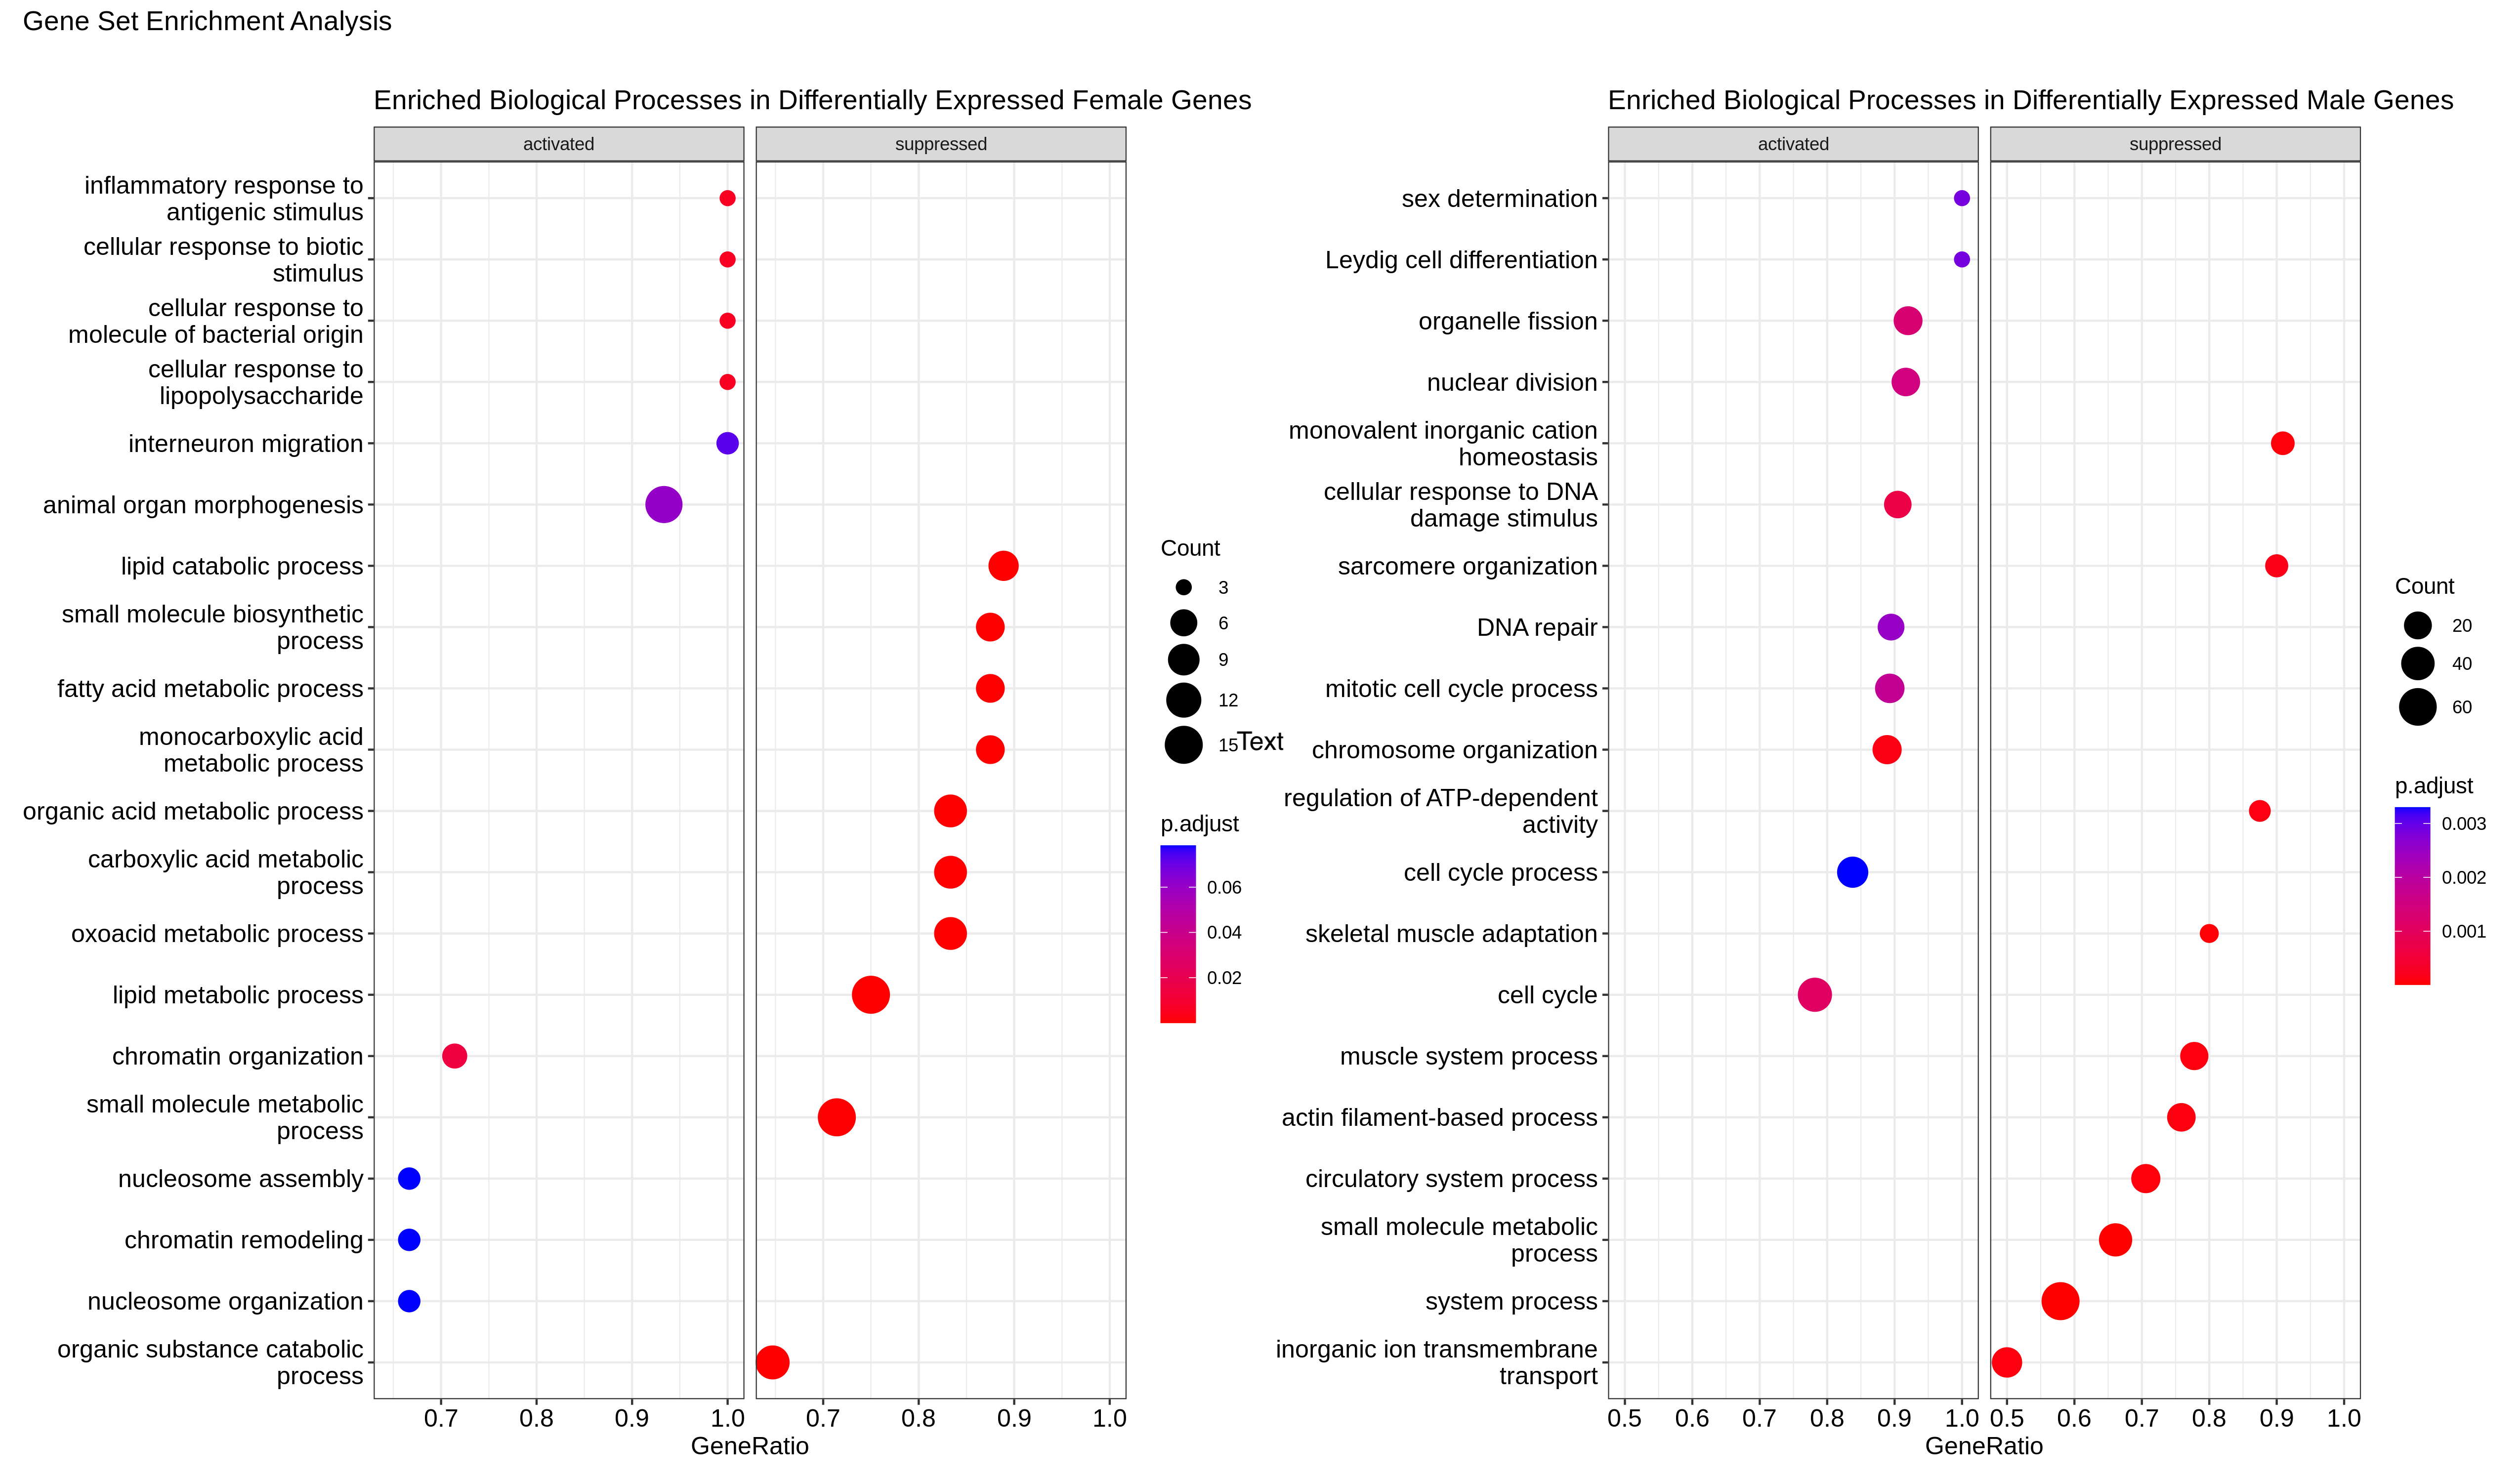
\includegraphics[width=\textwidth, height=11cm]{all_cancersgsea_exclusivedegenes_male_female_bp0.9.png}
		\caption{Dotplot showing the results of GSEA performed on EXCLUSIVELY differentially expressed genes (241 female, 638 male) found in females (left) and males (right). This example shows 10 activated and 10 suppressed enriched gene sets.}
		\label{fig:8}
	\end{figure}
	

	\subsection{Fishers Exact Test For Synthetic Lethality}
	
	\begin{figure}[!h]
		\centering
		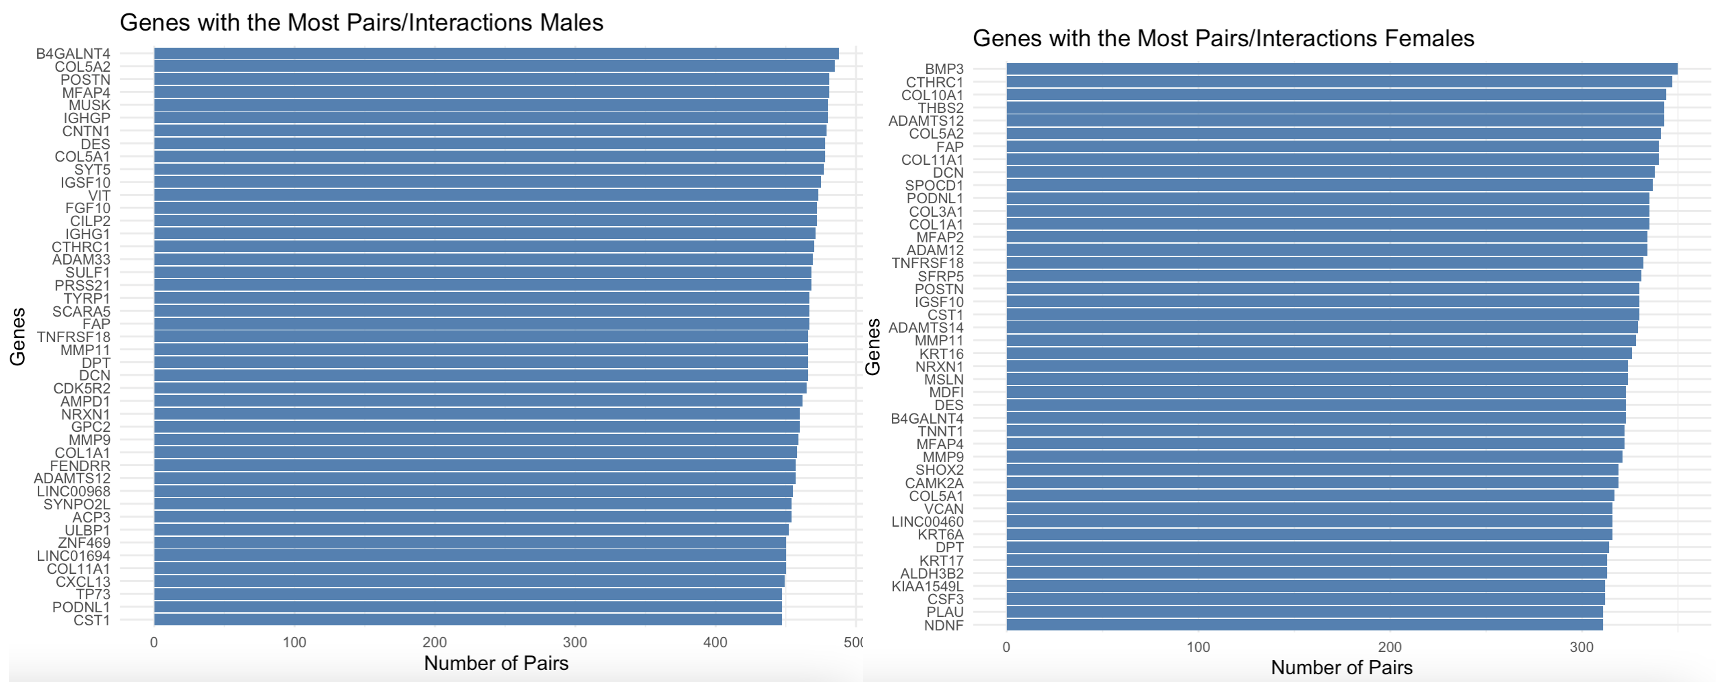
\includegraphics[width=\textwidth, height=8cm]{interactions.png}
		\caption{Barplot showing the genes involved in the most number of potential synthetic lethal pairs found using Fishers exact test}
		\label{fig:9}
	\end{figure}

\section{Next Steps/Future Avenues}
\begin{itemize}
	\item Build male and female synthetic lethal interaction networks using results from Fishers exact test. Use the genes as nodes and the odds ratios as edges to build the networks. (Packages: \texttt{NetworkX} Python, \texttt{pyvis} Python). Find differences in the male and female networks.
	\item Perform survival analysis on the SL pairs found using Fishers exact test and see which pairs contribute to improved patient survival. This could provide us with more clinically relevant synthetic lethal interactions.
	\item Incorporate other types of data. We only included RNA-seq data, what about copy number variation, methylation, etc... this could strengthen the validity of the study.
	\item Normal tissue proxy: There is a lack of normal tissue samples in the TCGA database. This restricted the number of cancer types we used in the study, as well as the sample size of the cancer types we did use. Can we use a different database to find matched samples? Can we use a machine learning approach to generate normal tissue expression data? Emailed the author of this paper, interesting stuff in terms of generating normal tissue expression but the author never got back to me with her code. \citep{zeng2019selecting}
	\item Do males have higher incidence of lung cancer because more of them are smokers, or is it because they are male. Can we try and better understand if other factors (like societal factors) cause sex differences, or is it truly due to genetic differences in sex?
	\item Menopause? Age Differences? Differences in medications?
\end{itemize}

%	\subsection{Assessing the Evolution Simulator}

%	\subsection{Applying the Simulator to an ABC-MCMC}

%\section{Discussion}

%	\subsection{Mutations Have the Ability to Destroy LCR Formation}

%	\subsection{Does the Length of a Repeat Play a Role in Insertions/Deletions}

%	\subsection{Why Parameters Could not be Estimated}

%	\subsection{Conclusion}

\clearpage\newpage
\section{Code \& Supplementary Materials (Transition Document)}

\hl{All of the following files listed are located on the Graham Cluster at} \texttt{$\sim$/projects/def-sushant/alextu/\newline slproject\_pmcrc}

\hl{Scripts used to obtain and format data can be found at} \texttt{$\sim$/projects/def-sushant/alextu/\newline slproject\_pmcrc/raw\_data/scripts}

\hl{Matching executables for these scripts can be found at} \texttt{$\sim$/projects/def-sushant/alextu/\newline slproject\_pmcrc/raw\_data/executions}

NOTE: THE NUMBERED ORDER THESE SCRIPTS APPEAR IN MATCHES THE ORDER IN WHICH THEY WERE RUN

\begin{enumerate}
\item\texttt{tcgabiolinks\_rawcount\_rnaseq\_download\_female.R} - SCRIPT

This script utilizes the tcgabiolinks package in R to retrieve gene expression data (RNA-seq) for a specific set of TCGA barcodes. The TCGA barcodes used in this script came from females of a specific cancer type. For each cancer type, a raw gene expression matrix is produced with genes as rows, and samples as columns. This is the first script run in the workflow in order to download the TCGA rna-seq data for the cancer types we were interested in.

RUN ON LOGIN NODE/LOCAL COMPUTER, NOT ON COMPUTE NODE, COMPUTE NODE CANT DOWNLOAD

\item\texttt{tcgabiolinks\_rawcount\_rnaseq\_download\_male.R} - SCRIPT

This script utilizes the tcgabiolinks package in R to retrieve gene expression data (RNA-seq) for a specific set of TCGA barcodes. The TCGA barcodes used in this script came from males of a specific cancer type. For each cancer type, a raw gene expression matrix is produced with genes as rows, and samples as columns. This is the first script run in the workflow in order to download the TCGA rna-seq data for the cancer types we were interested in.

RUN ON LOGIN NODE/LOCAL COMPUTER, NOT ON COMPUTE NODE, COMPUTE NODE CANT DOWNLOAD

\item\texttt{tcgabiolinks\_rawcount\_clinical\_download\_female.R} - SCRIPT

This script utilizes the tcgabiolinks package in R to retrieve clinical metadata for a specific set of TCGA barcodes. The TCGA barcodes used in this script came from females of a specific cancer type. For each cancer type, a SummarizedExperiment (R object) is produced and clinical information such as age at diagnosis and tissue of origin can be extracted.

RUN ON LOGIN NODE/LOCAL COMPUTER, NOT ON COMPUTE NODE, COMPUTE NODE CANT DOWNLOAD

\item\texttt{tcgabiolinks\_rawcount\_clinical\_download\_male.R} - SCRIPT

This script utilizes the tcgabiolinks package in R to retrieve clinical metadata for a specific set of TCGA barcodes. The TCGA barcodes used in this script came from males of a specific cancer type. For each cancer type, a SummarizedExperiment (R object) is produced and clinical information such as age at diagnosis and tissue of origin can be extracted.

RUN ON LOGIN NODE/LOCAL COMPUTER, NOT ON COMPUTE NODE, COMPUTE NODE CANT DOWNLOAD
\item\texttt{extract\_clinical\_data\_females.R} - SCRIPT\newline
\texttt{extract\_clinical\_data\_females.sh} - EXECUTABLE

This script extracts the clinical information of interest from the SummarizedExperiment (R object). We obtain barcode, tissue, and age information for females in the form of a dataframe.

\item\texttt{extract\_clinical\_data\_males.R}- SCRIPT\newline
\texttt{extract\_clinical\_data\_males.sh} - EXECUTABLE

This script extracts the clinical information of interest from the SummarizedExperiment (R object). We obtain barcode, tissue, and age information for males in the form of a dataframe.

\item\texttt{extract\_both\_tp\_nt\_samples\_females.R} - SCRIPT \newline
\texttt{extract\_both\_tp\_nt\_samples\_females.sh} - EXECUTABLE

This script finds all females within a TCGA cancer type who have BOTH normal and tumor samples. The script does not account for individuals with more than one match, meaning that the script will take all tumor and healthy samples pertaining to an individual, not just one pair. In some cases, individuals had two normal tissue samples. The output from this script is a gene expression matrix for each cancer type with only matched normal and tumor samples.

\item\texttt{extract\_both\_tp\_nt\_samples\_males.R} - SCRIPT \newline
\texttt{extract\_both\_tp\_nt\_samples\_males.sh} - EXECUTABLE

This script finds all males within a TCGA cancer type who have BOTH normal and tumor samples. The script does not account for individuals with more than one match, meaning that the script will take all tumor and healthy samples pertaining to an individual, not just one pair. In some cases, individuals had two normal tissue samples. The output from this script is a gene expression matrix for each cancer type with only matched normal and tumor samples.

\item\texttt{merge\_rawcounts\_both\_tp\_nt\_samples\_females.R} - SCRIPT \newline
\texttt{merge\_rawcounts\_both\_tp\_nt\_samples\_females.sh} - EXECUTABLE

This script takes the gene expression matrices (with matched Normal-tumor tissue samples) for females of each cancer type and merges them together to create a raw pan-cancer matrix with all 12 cancer types. Rows are genes and columns are samples.

\item\texttt{merge\_rawcounts\_both\_tp\_nt\_samples\_males.R} - SCRIPT \newline
\texttt{merge\_rawcounts\_both\_tp\_nt\_samples\_males.R} - EXECUTABLE

This script takes the gene expression matrices (with matched Normal-tumor tissue samples) for males of each cancer type and merges them together to create a raw pan-cancer matrix with all 12 cancer types. Rows are genes and columns are samples.

\hl{Scripts used to process and visualize data can be found at} \texttt{$\sim$/projects/def-sushant/alextu/\newline slproject\_pmcrc/processed\_data/scripts}

\hl{Matching executables for these scripts can be found at}
\texttt{$\sim$/projects/def-sushant/alextu/\newline slproject\_pmcrc/processed\_data/executions}


\item\texttt{deseq2\_extract\_normalized\_counts\_allcancers\_female.R} - SCRIPT\newline
\texttt{deseq2\_extract\_normalized\_counts\_allcancers\_female.sh} - EXECUTABLE
	
This script runs the differential gene expression analysis for females (through DESeq2) using the pan-cancer dataframe created from the last script above. This entails normalization of the expression data as well as hypothesis testing for each gene to determine whether expression is significantly different between tumor and normal tissue. This script also gathers all the metadata for the samples included in the pan-cancer matrix (condition (NT vs TP), cancer type, tissue type, age). Lastly, the script can account for different quantile thresholds set by the user. We filtered out genes with expression values less than some quantile value of overall gene expression. We tried 90th quantile and 50th quantile. The output from this script is a DESeq object that can be used to obtain differential gene expression information (raw counts, normalized counts, hypothesis test results for gene expression including log2FoldChange and adjusted p-values).
	
\item\texttt{deseq2\_extract\_normalized\_counts\_allcancers\_male.R} - SCRIPT\newline
\texttt{deseq2\_extract\_normalized\_counts\_allcancers\_male.sh} - EXECUTABLE
	
This script runs the differential gene expression analysis for males (through DESeq2) using the pan-cancer dataframe created from the last script above. This entails normalization of the expression data as well as hypothesis testing for each gene to determine whether expression is significantly different between tumor and normal tissue. This script also gathers all the metadata for the samples included in the pan-cancer matrix (condition (NT vs TP), cancer type, tissue type, age). Lastly, the script can account for different quantile thresholds set by the user. We filtered out genes with expression values less than some quantile value of overall gene expression. We tried 90th quantile and 50th quantile. The output from this script is a DESeq object that can be used to obtain differential gene expression information (raw counts, normalized counts, hypothesis test results for gene expression including log2FoldChange and adjusted p-values).
	
\item\texttt{deseq2\_preprocessing\_boxplots\_quantile\_prefiltering\_allcancers\_female.R} - SCRIPT\newline
\texttt{deseq2\_preprocessing\_boxplots\_quantile\_prefiltering\_allcancers\_female.sh} - EXECUTABLE
	
This script uses the DESeq object produced in the last step for females to extract raw and normalized gene counts for the pan-cancer matrix. The script creates boxplots showing raw counts before normalization vs normalized and transformed counts. Used to view the effects of normalization. The user can specify the quantile threshold value they would like to use in the script.
	
\item\texttt{deseq2\_preprocessing\_boxplots\_quantile\_prefiltering\_allcancers\_male.R} - SCRIPT \newline
\texttt{deseq2\_preprocessing\_boxplots\_quantile\_prefiltering\_allcancers\_male.sh} - EXECUTABLE
	
This script uses the DESeq object produced in the last step for males to extract raw and normalized gene counts for the pan-cancer matrix. The script creates boxplots showing raw counts before normalization vs normalized and transformed counts. Used to view the effects of normalization. The user can specify the quantile threshold value they would like to use in the script.

\item\texttt{pca\_analysis\_mergedcancers\_quantiles\_prefiltering.R} - SCRIPT\newline
\texttt{pca\_analysis\_mergedcancers\_quantiles\_prefiltering.sh} - EXECUTABLE

This script runs principal component analysis on the normalized count data for males AND females to detect sources of variation in the gene expression data. The user can specify the quantile threshold value they would like to use in the script.
	
\item\texttt{dge\_analysis\_deseq2.R}
	
This script performs a lot of tasks.

RUN ON LOGIN NODE/LOCAL COMPUTER, NOT ON COMPUTE NODE, COMPUTE NODE CANT DOWNLOAD
	
\item\texttt{gsea\_analysis\_postdeseq.R}
	
This script performs gene set enrichment analysis using \texttt{clusterProfiler}.

RUN ON LOGIN NODE/LOCAL COMPUTER, NOT ON COMPUTE NODE, COMPUTE NODE CANT DOWNLOAD
	
\item\texttt{npmanova.R}
	
This script performs a non parametric multivariate analysis of variance (NPMANOVA) in order to determine if differences between 
	
\end{enumerate}

\clearpage\newpage
\section{References}

%%%FIGURES%%%%%

%%%%PRINTING BIBLIOGRAPHY%%%%
\nocite{*}
\printbibliography[heading=none, sorting=nyt]
\newpage

%\section{Appendix 1: Low Complexity Region Evolution Simulator}
%\texttt{/home/alext/scratch/abcmcmc-thesis4c12/mutations\_2\_BG\_vecs.cpp}
%\lstinputlisting[language=c++]{../mutations_2_BG_vecs.cpp}
%\newpage

%\section{Appendix 2: ABC-MCMC in C++}
%\texttt{/home/alext/scratch/abcmcmc-thesis4c12/abcmcmc.cpp}
%\lstinputlisting[language=c++]{../abcmcmc.cpp}
%\newpage

%\section{Appendix 3: Simulated Protein Summary Statistics}
%\texttt{/home/alext/scratch/abcmcmc-thesis4c12/abcmcmc.cpp/simulated\_protein.cpp}
%\lstinputlisting[language=c++]{../simulated_protein.cpp}
%\newpage

%\section{Appendix 4: Euclidean Distance and Normlization of Vectors}
%\texttt{/home/alext/scratch/abcmcmc-thesis4c12/abcmcmc.cpp/distance2.cpp}
%\lstinputlisting[language=c++]{../distance2.cpp}
%\newpage

%\section{Appendix 5: One Sample t-test}
%\texttt{/home/alext/scratch/abcmcmc-thesis4c12/abcmcmc.cpp/ttest.cpp}
%\lstinputlisting[language=c++]{../ttest.cpp}
%\newpage

\end{document}



